
% Inherit from the specified cell style.

% Default to the notebook output style

    


% Inherit from the specified cell style.




    
\documentclass[letter]{article}

    
    
\usepackage[T1]{fontenc}
% Nicer default font (+ math font) than Computer Modern for most use cases
\usepackage{mathpazo}

% Basic figure setup, for now with no caption control since it's done
% automatically by Pandoc (which extracts ![](path) syntax from Markdown).
\usepackage{graphicx}
% We will generate all images so they have a width \maxwidth. This means
% that they will get their normal width if they fit onto the page, but
% are scaled down if they would overflow the margins.
\makeatletter
\def\maxwidth{\ifdim\Gin@nat@width>\linewidth\linewidth
\else\Gin@nat@width\fi}
\makeatother
\let\Oldincludegraphics\includegraphics
% Set max figure width to be 80% of text width, for now hardcoded.
\renewcommand{\includegraphics}[1]{\Oldincludegraphics[width=.8\maxwidth]{#1}}
% Ensure that by default, figures have no caption (until we provide a
% proper Figure object with a Caption API and a way to capture that
% in the conversion process - todo).
% \usepackage{caption}
% \DeclareCaptionLabelFormat{nolabel}{}
% \captionsetup{labelformat=nolabel}

\usepackage{adjustbox} % Used to constrain images to a maximum size 
\usepackage{xcolor} % Allow colors to be defined
\usepackage{enumerate} % Needed for markdown enumerations to work
\usepackage{geometry} % Used to adjust the document margins
\usepackage{amsmath} % Equations
\usepackage{amssymb} % Equations
\usepackage{textcomp} % defines textquotesingle
% Hack from http://tex.stackexchange.com/a/47451/13684:
\AtBeginDocument{%
    \def\PYZsq{\textquotesingle}% Upright quotes in Pygmentized code
}
\usepackage{upquote} % Upright quotes for verbatim code
\usepackage{eurosym} % defines \euro
\usepackage[mathletters]{ucs} % Extended unicode (utf-8) support
\usepackage[utf8x]{inputenc} % Allow utf-8 characters in the tex document
\usepackage{fancyvrb} % verbatim replacement that allows latex
\usepackage{grffile} % extends the file name processing of package graphics 
                     % to support a larger range 
% The hyperref package gives us a pdf with properly built
% internal navigation ('pdf bookmarks' for the table of contents,
% internal cross-reference links, web links for URLs, etc.)
\usepackage{hyperref}
\usepackage{longtable} % longtable support required by pandoc >1.10
\usepackage{booktabs}  % table support for pandoc > 1.12.2
\usepackage[inline]{enumitem} % IRkernel/repr support (it uses the enumerate* environment)
\usepackage[normalem]{ulem} % ulem is needed to support strikethroughs (\sout)
                            % normalem makes italics be italics, not underlines

\usepackage{natbib}
\usepackage[scr]{rsfso}
\usepackage{bm}
\usepackage{eulervm}
\usepackage{lineno}


    
    
    
    % Colors for the hyperref package
    \definecolor{urlcolor}{rgb}{0,.145,.698}
    \definecolor{linkcolor}{rgb}{.71,0.21,0.01}
    \definecolor{citecolor}{rgb}{.12,.54,.11}

    % ANSI colors
    \definecolor{ansi-black}{HTML}{3E424D}
    \definecolor{ansi-black-intense}{HTML}{282C36}
    \definecolor{ansi-red}{HTML}{E75C58}
    \definecolor{ansi-red-intense}{HTML}{B22B31}
    \definecolor{ansi-green}{HTML}{00A250}
    \definecolor{ansi-green-intense}{HTML}{007427}
    \definecolor{ansi-yellow}{HTML}{DDB62B}
    \definecolor{ansi-yellow-intense}{HTML}{B27D12}
    \definecolor{ansi-blue}{HTML}{208FFB}
    \definecolor{ansi-blue-intense}{HTML}{0065CA}
    \definecolor{ansi-magenta}{HTML}{D160C4}
    \definecolor{ansi-magenta-intense}{HTML}{A03196}
    \definecolor{ansi-cyan}{HTML}{60C6C8}
    \definecolor{ansi-cyan-intense}{HTML}{258F8F}
    \definecolor{ansi-white}{HTML}{C5C1B4}
    \definecolor{ansi-white-intense}{HTML}{A1A6B2}

    % commands and environments needed by pandoc snippets
    % extracted from the output of `pandoc -s`
    \providecommand{\tightlist}{%
      \setlength{\itemsep}{0pt}\setlength{\parskip}{0pt}}
    \DefineVerbatimEnvironment{Highlighting}{Verbatim}{commandchars=\\\{\}}
    % Add ',fontsize=\small' for more characters per line
    \newenvironment{Shaded}{}{}
    \newcommand{\KeywordTok}[1]{\textcolor[rgb]{0.00,0.44,0.13}{\textbf{{#1}}}}
    \newcommand{\DataTypeTok}[1]{\textcolor[rgb]{0.56,0.13,0.00}{{#1}}}
    \newcommand{\DecValTok}[1]{\textcolor[rgb]{0.25,0.63,0.44}{{#1}}}
    \newcommand{\BaseNTok}[1]{\textcolor[rgb]{0.25,0.63,0.44}{{#1}}}
    \newcommand{\FloatTok}[1]{\textcolor[rgb]{0.25,0.63,0.44}{{#1}}}
    \newcommand{\CharTok}[1]{\textcolor[rgb]{0.25,0.44,0.63}{{#1}}}
    \newcommand{\StringTok}[1]{\textcolor[rgb]{0.25,0.44,0.63}{{#1}}}
    \newcommand{\CommentTok}[1]{\textcolor[rgb]{0.38,0.63,0.69}{\textit{{#1}}}}
    \newcommand{\OtherTok}[1]{\textcolor[rgb]{0.00,0.44,0.13}{{#1}}}
    \newcommand{\AlertTok}[1]{\textcolor[rgb]{1.00,0.00,0.00}{\textbf{{#1}}}}
    \newcommand{\FunctionTok}[1]{\textcolor[rgb]{0.02,0.16,0.49}{{#1}}}
    \newcommand{\RegionMarkerTok}[1]{{#1}}
    \newcommand{\ErrorTok}[1]{\textcolor[rgb]{1.00,0.00,0.00}{\textbf{{#1}}}}
    \newcommand{\NormalTok}[1]{{#1}}
    
    % Additional commands for more recent versions of Pandoc
    \newcommand{\ConstantTok}[1]{\textcolor[rgb]{0.53,0.00,0.00}{{#1}}}
    \newcommand{\SpecialCharTok}[1]{\textcolor[rgb]{0.25,0.44,0.63}{{#1}}}
    \newcommand{\VerbatimStringTok}[1]{\textcolor[rgb]{0.25,0.44,0.63}{{#1}}}
    \newcommand{\SpecialStringTok}[1]{\textcolor[rgb]{0.73,0.40,0.53}{{#1}}}
    \newcommand{\ImportTok}[1]{{#1}}
    \newcommand{\DocumentationTok}[1]{\textcolor[rgb]{0.73,0.13,0.13}{\textit{{#1}}}}
    \newcommand{\AnnotationTok}[1]{\textcolor[rgb]{0.38,0.63,0.69}{\textbf{\textit{{#1}}}}}
    \newcommand{\CommentVarTok}[1]{\textcolor[rgb]{0.38,0.63,0.69}{\textbf{\textit{{#1}}}}}
    \newcommand{\VariableTok}[1]{\textcolor[rgb]{0.10,0.09,0.49}{{#1}}}
    \newcommand{\ControlFlowTok}[1]{\textcolor[rgb]{0.00,0.44,0.13}{\textbf{{#1}}}}
    \newcommand{\OperatorTok}[1]{\textcolor[rgb]{0.40,0.40,0.40}{{#1}}}
    \newcommand{\BuiltInTok}[1]{{#1}}
    \newcommand{\ExtensionTok}[1]{{#1}}
    \newcommand{\PreprocessorTok}[1]{\textcolor[rgb]{0.74,0.48,0.00}{{#1}}}
    \newcommand{\AttributeTok}[1]{\textcolor[rgb]{0.49,0.56,0.16}{{#1}}}
    \newcommand{\InformationTok}[1]{\textcolor[rgb]{0.38,0.63,0.69}{\textbf{\textit{{#1}}}}}
    \newcommand{\WarningTok}[1]{\textcolor[rgb]{0.38,0.63,0.69}{\textbf{\textit{{#1}}}}}
    
    
    % Define a nice break command that doesn't care if a line doesn't already
    % exist.
    \def\br{\hspace*{\fill} \\* }
    % Math Jax compatability definitions
    \def\gt{>}
    \def\lt{<}
    % Document parameters
    \title{GeoRDD manuscript}
    
    \author{Maxime Rischard}
    

    % Pygments definitions
    
\makeatletter
\def\PY@reset{\let\PY@it=\relax \let\PY@bf=\relax%
    \let\PY@ul=\relax \let\PY@tc=\relax%
    \let\PY@bc=\relax \let\PY@ff=\relax}
\def\PY@tok#1{\csname PY@tok@#1\endcsname}
\def\PY@toks#1+{\ifx\relax#1\empty\else%
    \PY@tok{#1}\expandafter\PY@toks\fi}
\def\PY@do#1{\PY@bc{\PY@tc{\PY@ul{%
    \PY@it{\PY@bf{\PY@ff{#1}}}}}}}
\def\PY#1#2{\PY@reset\PY@toks#1+\relax+\PY@do{#2}}

\expandafter\def\csname PY@tok@gp\endcsname{\let\PY@bf=\textbf\def\PY@tc##1{\textcolor[rgb]{0.00,0.00,0.50}{##1}}}
\expandafter\def\csname PY@tok@nt\endcsname{\let\PY@bf=\textbf\def\PY@tc##1{\textcolor[rgb]{0.00,0.50,0.00}{##1}}}
\expandafter\def\csname PY@tok@kd\endcsname{\let\PY@bf=\textbf\def\PY@tc##1{\textcolor[rgb]{0.00,0.50,0.00}{##1}}}
\expandafter\def\csname PY@tok@mf\endcsname{\def\PY@tc##1{\textcolor[rgb]{0.40,0.40,0.40}{##1}}}
\expandafter\def\csname PY@tok@w\endcsname{\def\PY@tc##1{\textcolor[rgb]{0.73,0.73,0.73}{##1}}}
\expandafter\def\csname PY@tok@sd\endcsname{\let\PY@it=\textit\def\PY@tc##1{\textcolor[rgb]{0.73,0.13,0.13}{##1}}}
\expandafter\def\csname PY@tok@mb\endcsname{\def\PY@tc##1{\textcolor[rgb]{0.40,0.40,0.40}{##1}}}
\expandafter\def\csname PY@tok@gd\endcsname{\def\PY@tc##1{\textcolor[rgb]{0.63,0.00,0.00}{##1}}}
\expandafter\def\csname PY@tok@no\endcsname{\def\PY@tc##1{\textcolor[rgb]{0.53,0.00,0.00}{##1}}}
\expandafter\def\csname PY@tok@kt\endcsname{\def\PY@tc##1{\textcolor[rgb]{0.69,0.00,0.25}{##1}}}
\expandafter\def\csname PY@tok@kr\endcsname{\let\PY@bf=\textbf\def\PY@tc##1{\textcolor[rgb]{0.00,0.50,0.00}{##1}}}
\expandafter\def\csname PY@tok@vm\endcsname{\def\PY@tc##1{\textcolor[rgb]{0.10,0.09,0.49}{##1}}}
\expandafter\def\csname PY@tok@sa\endcsname{\def\PY@tc##1{\textcolor[rgb]{0.73,0.13,0.13}{##1}}}
\expandafter\def\csname PY@tok@nv\endcsname{\def\PY@tc##1{\textcolor[rgb]{0.10,0.09,0.49}{##1}}}
\expandafter\def\csname PY@tok@na\endcsname{\def\PY@tc##1{\textcolor[rgb]{0.49,0.56,0.16}{##1}}}
\expandafter\def\csname PY@tok@s\endcsname{\def\PY@tc##1{\textcolor[rgb]{0.73,0.13,0.13}{##1}}}
\expandafter\def\csname PY@tok@sh\endcsname{\def\PY@tc##1{\textcolor[rgb]{0.73,0.13,0.13}{##1}}}
\expandafter\def\csname PY@tok@sc\endcsname{\def\PY@tc##1{\textcolor[rgb]{0.73,0.13,0.13}{##1}}}
\expandafter\def\csname PY@tok@gh\endcsname{\let\PY@bf=\textbf\def\PY@tc##1{\textcolor[rgb]{0.00,0.00,0.50}{##1}}}
\expandafter\def\csname PY@tok@nf\endcsname{\def\PY@tc##1{\textcolor[rgb]{0.00,0.00,1.00}{##1}}}
\expandafter\def\csname PY@tok@nb\endcsname{\def\PY@tc##1{\textcolor[rgb]{0.00,0.50,0.00}{##1}}}
\expandafter\def\csname PY@tok@mh\endcsname{\def\PY@tc##1{\textcolor[rgb]{0.40,0.40,0.40}{##1}}}
\expandafter\def\csname PY@tok@gr\endcsname{\def\PY@tc##1{\textcolor[rgb]{1.00,0.00,0.00}{##1}}}
\expandafter\def\csname PY@tok@cm\endcsname{\let\PY@it=\textit\def\PY@tc##1{\textcolor[rgb]{0.25,0.50,0.50}{##1}}}
\expandafter\def\csname PY@tok@nd\endcsname{\def\PY@tc##1{\textcolor[rgb]{0.67,0.13,1.00}{##1}}}
\expandafter\def\csname PY@tok@gt\endcsname{\def\PY@tc##1{\textcolor[rgb]{0.00,0.27,0.87}{##1}}}
\expandafter\def\csname PY@tok@ne\endcsname{\let\PY@bf=\textbf\def\PY@tc##1{\textcolor[rgb]{0.82,0.25,0.23}{##1}}}
\expandafter\def\csname PY@tok@s2\endcsname{\def\PY@tc##1{\textcolor[rgb]{0.73,0.13,0.13}{##1}}}
\expandafter\def\csname PY@tok@nl\endcsname{\def\PY@tc##1{\textcolor[rgb]{0.63,0.63,0.00}{##1}}}
\expandafter\def\csname PY@tok@ch\endcsname{\let\PY@it=\textit\def\PY@tc##1{\textcolor[rgb]{0.25,0.50,0.50}{##1}}}
\expandafter\def\csname PY@tok@sb\endcsname{\def\PY@tc##1{\textcolor[rgb]{0.73,0.13,0.13}{##1}}}
\expandafter\def\csname PY@tok@err\endcsname{\def\PY@bc##1{\setlength{\fboxsep}{0pt}\fcolorbox[rgb]{1.00,0.00,0.00}{1,1,1}{\strut ##1}}}
\expandafter\def\csname PY@tok@bp\endcsname{\def\PY@tc##1{\textcolor[rgb]{0.00,0.50,0.00}{##1}}}
\expandafter\def\csname PY@tok@si\endcsname{\let\PY@bf=\textbf\def\PY@tc##1{\textcolor[rgb]{0.73,0.40,0.53}{##1}}}
\expandafter\def\csname PY@tok@sr\endcsname{\def\PY@tc##1{\textcolor[rgb]{0.73,0.40,0.53}{##1}}}
\expandafter\def\csname PY@tok@ge\endcsname{\let\PY@it=\textit}
\expandafter\def\csname PY@tok@go\endcsname{\def\PY@tc##1{\textcolor[rgb]{0.53,0.53,0.53}{##1}}}
\expandafter\def\csname PY@tok@gs\endcsname{\let\PY@bf=\textbf}
\expandafter\def\csname PY@tok@dl\endcsname{\def\PY@tc##1{\textcolor[rgb]{0.73,0.13,0.13}{##1}}}
\expandafter\def\csname PY@tok@c1\endcsname{\let\PY@it=\textit\def\PY@tc##1{\textcolor[rgb]{0.25,0.50,0.50}{##1}}}
\expandafter\def\csname PY@tok@cpf\endcsname{\let\PY@it=\textit\def\PY@tc##1{\textcolor[rgb]{0.25,0.50,0.50}{##1}}}
\expandafter\def\csname PY@tok@mi\endcsname{\def\PY@tc##1{\textcolor[rgb]{0.40,0.40,0.40}{##1}}}
\expandafter\def\csname PY@tok@fm\endcsname{\def\PY@tc##1{\textcolor[rgb]{0.00,0.00,1.00}{##1}}}
\expandafter\def\csname PY@tok@se\endcsname{\let\PY@bf=\textbf\def\PY@tc##1{\textcolor[rgb]{0.73,0.40,0.13}{##1}}}
\expandafter\def\csname PY@tok@gu\endcsname{\let\PY@bf=\textbf\def\PY@tc##1{\textcolor[rgb]{0.50,0.00,0.50}{##1}}}
\expandafter\def\csname PY@tok@ow\endcsname{\let\PY@bf=\textbf\def\PY@tc##1{\textcolor[rgb]{0.67,0.13,1.00}{##1}}}
\expandafter\def\csname PY@tok@cp\endcsname{\def\PY@tc##1{\textcolor[rgb]{0.74,0.48,0.00}{##1}}}
\expandafter\def\csname PY@tok@il\endcsname{\def\PY@tc##1{\textcolor[rgb]{0.40,0.40,0.40}{##1}}}
\expandafter\def\csname PY@tok@nn\endcsname{\let\PY@bf=\textbf\def\PY@tc##1{\textcolor[rgb]{0.00,0.00,1.00}{##1}}}
\expandafter\def\csname PY@tok@sx\endcsname{\def\PY@tc##1{\textcolor[rgb]{0.00,0.50,0.00}{##1}}}
\expandafter\def\csname PY@tok@k\endcsname{\let\PY@bf=\textbf\def\PY@tc##1{\textcolor[rgb]{0.00,0.50,0.00}{##1}}}
\expandafter\def\csname PY@tok@ss\endcsname{\def\PY@tc##1{\textcolor[rgb]{0.10,0.09,0.49}{##1}}}
\expandafter\def\csname PY@tok@gi\endcsname{\def\PY@tc##1{\textcolor[rgb]{0.00,0.63,0.00}{##1}}}
\expandafter\def\csname PY@tok@vg\endcsname{\def\PY@tc##1{\textcolor[rgb]{0.10,0.09,0.49}{##1}}}
\expandafter\def\csname PY@tok@m\endcsname{\def\PY@tc##1{\textcolor[rgb]{0.40,0.40,0.40}{##1}}}
\expandafter\def\csname PY@tok@vc\endcsname{\def\PY@tc##1{\textcolor[rgb]{0.10,0.09,0.49}{##1}}}
\expandafter\def\csname PY@tok@c\endcsname{\let\PY@it=\textit\def\PY@tc##1{\textcolor[rgb]{0.25,0.50,0.50}{##1}}}
\expandafter\def\csname PY@tok@mo\endcsname{\def\PY@tc##1{\textcolor[rgb]{0.40,0.40,0.40}{##1}}}
\expandafter\def\csname PY@tok@kc\endcsname{\let\PY@bf=\textbf\def\PY@tc##1{\textcolor[rgb]{0.00,0.50,0.00}{##1}}}
\expandafter\def\csname PY@tok@s1\endcsname{\def\PY@tc##1{\textcolor[rgb]{0.73,0.13,0.13}{##1}}}
\expandafter\def\csname PY@tok@cs\endcsname{\let\PY@it=\textit\def\PY@tc##1{\textcolor[rgb]{0.25,0.50,0.50}{##1}}}
\expandafter\def\csname PY@tok@vi\endcsname{\def\PY@tc##1{\textcolor[rgb]{0.10,0.09,0.49}{##1}}}
\expandafter\def\csname PY@tok@o\endcsname{\def\PY@tc##1{\textcolor[rgb]{0.40,0.40,0.40}{##1}}}
\expandafter\def\csname PY@tok@nc\endcsname{\let\PY@bf=\textbf\def\PY@tc##1{\textcolor[rgb]{0.00,0.00,1.00}{##1}}}
\expandafter\def\csname PY@tok@kn\endcsname{\let\PY@bf=\textbf\def\PY@tc##1{\textcolor[rgb]{0.00,0.50,0.00}{##1}}}
\expandafter\def\csname PY@tok@ni\endcsname{\let\PY@bf=\textbf\def\PY@tc##1{\textcolor[rgb]{0.60,0.60,0.60}{##1}}}
\expandafter\def\csname PY@tok@kp\endcsname{\def\PY@tc##1{\textcolor[rgb]{0.00,0.50,0.00}{##1}}}

\def\PYZbs{\char`\\}
\def\PYZus{\char`\_}
\def\PYZob{\char`\{}
\def\PYZcb{\char`\}}
\def\PYZca{\char`\^}
\def\PYZam{\char`\&}
\def\PYZlt{\char`\<}
\def\PYZgt{\char`\>}
\def\PYZsh{\char`\#}
\def\PYZpc{\char`\%}
\def\PYZdl{\char`\$}
\def\PYZhy{\char`\-}
\def\PYZsq{\char`\'}
\def\PYZdq{\char`\"}
\def\PYZti{\char`\~}
% for compatibility with earlier versions
\def\PYZat{@}
\def\PYZlb{[}
\def\PYZrb{]}
\makeatother


    % Exact colors from NB
    \definecolor{incolor}{rgb}{0.0, 0.0, 0.5}
    \definecolor{outcolor}{rgb}{0.545, 0.0, 0.0}


    \newcommand{\genericdel}[3]{%
      \left#1#3\right#2
    }
    \newcommand{\del}[1]{\genericdel(){#1}}
    \newcommand{\sbr}[1]{\genericdel[]{#1}}
    \newcommand{\cbr}[1]{\genericdel\{\}{#1}}
    \DeclareMathOperator*{\argmin}{arg\,min}
    \DeclareMathOperator*{\argmax}{arg\,max}
	\let\Pr\relax
    \DeclareMathOperator{\Pr}{\mathbb{P}}
    \DeclareMathOperator{\E}{\mathbb{E}}
    \DeclareMathOperator{\V}{\mathbb{V}}
    \DeclareMathOperator{\cov}{{cov}}
    \DeclareMathOperator{\var}{{var}}
    \DeclareMathOperator{\Ind}{\mathbb{I}}
	\DeclareMathOperator*{\sgn}{{sgn}}

    \DeclareMathOperator{\normal}{\mathcal{N}}
    \DeclareMathOperator{\unif}{Uniform}
    \DeclareMathOperator{\invchi}{\mathrm{Inv-\chi}^2}

    \newcommand{\abs}[1]{\genericdel||{#1}}
    \newcommand{\effect}{\mathrm{eff}}
    \newcommand{\xtilde}{\widetilde{X}}
    \newcommand{\boxleft}{\squareleftblack}
    \newcommand{\boxright}{\squarerightblack}
    \newcommand{\discont}{\boxbar}
    \newcommand{\jleft}{\unicode{x21E5}}
    \newcommand{\jright}{\unicode{x21E4}}

    \DeclareMathOperator{\ones}{\mathbf{1}}
    \DeclareUnicodeCharacter{9707}{$\boxbar$}
    
    \DeclareMathOperator{\GP}{\mathcal{GP}}
    \DeclareMathOperator{\scrl}{\mathscr{l}}
    \newcommand{\saleprice}{\mathtt{SalePrice}}
    \newcommand{\sqft}{\mathtt{SQFT}}
    
    \newcommand{\tax}{\mathtt{TaxClass}}
    \newcommand{\building}{\mathtt{BuildingClass}}
    \newcommand{\district}{\mathtt{District}}

    \newcommand{\gp}{\mathcal{GP}}
    \newcommand{\trans}{^{\intercal}}
    \newcommand{\scrS}{\mathscr{S}}
    \newcommand{\sigmaf}{\sigma_{\mathrm{GP}}}
    \newcommand{\sigman}{\sigma_{\epsilon}}
    \newcommand{\sigmatau}{\sigma_{\tau}}
    \newcommand{\sigmabeta}{\sigma_{\beta}}
    \newcommand{\sigmamu}{\sigma_{\mu}}
    \newcommand{\sigmagamma}{\sigma_{\gamma}}
    \newcommand{\svec}{\mathbold{s}}
    \newcommand{\dvec}{\mathbold{d}}
    \newcommand{\xvec}{\mathbold{x}}
    \newcommand{\yvec}{\mathbold{y}}
    \newcommand{\vvec}{\mathbold{v}}
    \newcommand{\muvec}{\mathbold{\mu}}
    \newcommand{\indep}{\protect\mathpalette{\protect\independenT}{\perp}}
	\def\independenT#1#2{\mathrel{\rlap{$#1#2$}\mkern2mu{#1#2}}}
    \newcommand{\iid}{iid}
    \newcommand{\vectreat}{\Ind_{T}}

    \newcommand{\boundary}{\partial}
    \newcommand{\sentinels}{\bm{\boundary}}
    \newcommand{\eye}{\mathbf{I}}
    \newcommand{\K}{\mathbf{K}}

    \DeclareMathOperator{\trace}{trace}
    \newcommand{\linavg}{\bar{\tau}}
    \newcommand{\invvar}{\tau^{IV}}
    \newcommand{\modnull}{\mathscr{M}_0}
    \newcommand{\modalt}{\mathscr{M}_1}
    \newcommand{\degree}{{\,^\circ}}

	\providecommand{\tightlist}{%
  	  \setlength{\itemsep}{0pt}\setlength{\parskip}{0pt}}
	\renewcommand{\cite}[1]{\citep{#1}}


    
    % Prevent overflowing lines due to hard-to-break entities
    \sloppy 
    % Setup hyperref package
    \hypersetup{
      breaklinks=true,  % so long urls are correctly broken across lines
      colorlinks=true,
      urlcolor=urlcolor,
      linkcolor=linkcolor,
      citecolor=citecolor,
      }
    % Slightly bigger margins than the latex defaults
    
    \geometry{verbose,tmargin=1in,bmargin=1in,lmargin=1in,rmargin=1in}
    
    

    \begin{document}
    
    
    
    \maketitle
    
    
	\tableofcontents


    





    	\section{Introduction}\label{introduction}

\begin{itemize}
\tightlist
\item
  Problem we're trying to solve

  \begin{itemize}
  \tightlist
  \item
    treatment applied to one region and not a neighboring region
  \item
    with no overlap
  \item
    how to estimate the causal effect of the treatment?
  \item
    if the outcome is not spatially varying, there's no problem
  \item
    otherwise, the treatment is confounded with location
  \end{itemize}
\item
  In 1D, this is recognied as a regression discontinuity design

  \begin{itemize}
  \tightlist
  \item
    which is now a well-established methodology {[}citations{]}
  \item
    and comes with a causal inference story {[}Imbens{]}
  \end{itemize}
\item
  In spatial settings, practicioners therefore attempt to use these tools

  \begin{itemize}
  \tightlist
  \item
    but they don't generalize easily to 2D
  \item
    so often end up projecting onto distance from boundary
  \end{itemize}
\item
  We think this is a bad idea

  \begin{itemize}
  \tightlist
  \item
    ignores spatial structure / correlation
  \item
    low power and could get the wrong answer
  \end{itemize}
\item
  Mention some of the more sophisticated approaches to this same problem {[}Keele{]}

  \begin{itemize}
  \tightlist
  \item
    maybe briefly mention why we don't like them
  \end{itemize}
\item
  Our approach: framework analogous to 1D RDD

  \begin{itemize}
  \tightlist
  \item
    1D:

    \begin{enumerate}
    \def\labelenumi{\arabic{enumi}.}
    \tightlist
    \item
      fit the outcome \textbf{function} on both sides
    \item
      extrapolate to the \textbf{discontinuity point} \(x*\)
    \item
      take difference to obtain \(\tau(x*) \in \mathbb{R}\)
    \end{enumerate}
  \item
    2D:

    \begin{enumerate}
    \def\labelenumi{\arabic{enumi}.}
    \tightlist
    \item
      fit the outcome \textbf{surface} on both sides
    \item
      extrapolate to \textbf{boundary curve} \(\boundary\)
    \item
      take difference to obtain \(\tau(\boundary): \mathbb{R} \rightarrow \mathbb{R}\) {[}help with notation? or is this too mathematical anyway?{]}
    \end{enumerate}
  \end{itemize}
\item
  Challenge 1: functional estimand is unusual
\item
  Challenge 2: how to fit surface on both sides

  \begin{itemize}
  \tightlist
  \item
    in this framework there is not restriction on how surface fitting and extrapolation are performed
  \item
    in 1D RDD, local linear regression has become standard

    \begin{itemize}
    \tightlist
    \item
      though other options have been explored (like splines?)
    \end{itemize}
  \item
    but this isn't suitable in 2D
  \end{itemize}
\item
  Challenge 3: summarizing functional estimand

  \begin{itemize}
  \tightlist
  \item
    how to take an average?
  \item
    1D manifold embedded in 2D space poses problems
  \item
    pitfalls detailed in Section X
  \end{itemize}
\item
  Challenge 4: hypothesis testing on functional estimand
\item
  We use Gaussian processes (kriging), which are widespread in spatial statistics

  \begin{itemize}
  \tightlist
  \item
    many advantages

    \begin{itemize}
    \tightlist
    \item
      flexible
    \item
      known to perform well in spatial settings
    \item
      analytic solutions
    \end{itemize}
  \end{itemize}
\item
  we explore and address the 4 challenges using GPs
\item
  by the way, GP's can also be used in 1D {[}cite Zach{]}
\end{itemize}
    


    	Consider an experiment performed on a population of units that are distributed geographically,
in which a treatment gets applied to selected units, while the rest are used as a control group.
We then measure an outcome of interest, \(Y_i\).
If the treatment assignment is randomized, standard estimators from randomized control trials apply, such as the difference in observed means within the treatment and control groups.
If outcomes vary spatially, it would be advisable to match units that are near each other, in order to prevent this variation from confounding the estimate {[}a citation here would be nice{]}.

Now, we may find ourselves in a situation where the treatment does not get assigned at random.
Instead, the land is arbitrarily divided into two contiguous regions, and the treatment applied to units in one region, and withheld from those in the other.
Ignoring the spatial covariates is particularly inadvisable in this scenario, as units in the two regions could be very different from each other.
Matching is no longer viable either, as there is no overlap in the spatial covariates.

Examples of this situation occasionally appear in the literature. In \cite{macdonald2015effect}, a private police force patrols a neighborhood, but stays out of surrounding areas, and a causal effect on crime rates is sought. In \cite{chen2013evidence}, a policy applies South of the Huai River in China but not in the North, and pollution levels and life expectancies are measured to infer environmental and health impacts of the policy.

When treatment assignment is dictated by thresholding a single covariate (above or below the threshold all units are assigned to treatment, and all others to control), then the methodologies developed for regression discontinuity designs (RDD) enable the estimation of a causal effect despite the lack of overlap in the covariate. Our aim is to develop methodologies for our setting, which we recognize as geographic regression discontinuity designs \cite{keele_titiunik_2015}.

Noticing this connection, practicioners often wish to use the well-established tools developed for one-dimensional RDDs for their spatial problem.
Unfortunately, the most common methodologies, based on local linear regression on both sides of the boundary, do not extend naturally to two-dimensional settings.
A temptation therefore arises to reduce a geographic RDD problem to a classical (one-dimensional) RDD by projecting locations onto the distance away from the boundary.
This is the approach taken by, for example, \cite{macdonald2015effect} and \cite{chen2013evidence}. \cite{keele_titiunik_2015} recognize the limitations of the Euclidian distance projection, and\ldots{}

{[}why this is a bad idea{]}
    


    	We propose a framework for analysing geographical regression discontinuity designs that is directly analogous to their univariate counterpart, and avoids the need to project positions onto a single dimension.
Univariate RDD methodologies can be abstracted to three steps:\\
1. Fit a smooth \textbf{function} to the outcomes against the covariate on each side of the discontinuity;
2. Extrapolate the functions to the \textbf{discontinuity point} \(x^*\); and
3. Subtract the two extrapolations to obtain the estimated treatment effect \(\hat\tau(x^*) \in \mathbb{R}\).\\
Reusing the same conceptual skeleton and applying it to geographical RDDs, our framework proceeds analogously:\\
1. Fit a smooth \textbf{surface} to the outcomes against the geographical covariates on each side of the discontinuity;
2. Extrapolate the surfaces to the \textbf{boundary curve} \(\boundary\); and
3. Subtract the two extrapolations to obtain the estimated treatment effect along the boundary \(\hat\tau: \boundary \rightarrow \mathbb{R}\).
    


    	\section{Model Specification}\label{model-specification}

\subsection{Notation}\label{notation}

\begin{itemize}
\tightlist
\item
  2-dimensional coordinate space \(\scrS\)
\item
  treatment units are in region \(\scrS_T \subset \scrS\) and control units are in non-overlapping \(\scrS_C\) outside of the treatment region, so that \(\scrS_C = \scrS_T^c\) and \(\scrS_T \cup \scrS_C = \scrS\)
\item
  Observed outcomes for units in treatment region are labeled \(Y_i = Y_T(\svec_i)\), and units in control region \(Y_i = Y_C(\svec_i)\).
\item
  Potential outcomes framework: Each unit has a potential outcome under treatment \(Y_T(\svec)\) and a potential outcome under control \(Y_C(\svec)\). If \(\svec \in \scrS_T\), then \(Y_T(\svec)\) is observed, otherwise \(Y_C(\svec)\) is observed.
\end{itemize}

\subsection{1GP solution}\label{gp-solution}

Most straightforwardly, we model the observed outcomes \(Y\) at locations \(S\) (an \(n \times 2\) matrix) as the sum of an intercept \(\mu\), linear trend \(S\beta\), a spatial Gaussian process \(f(S)\), a constant treatment effect \(\tau\) in the treatment region, and iid normal noise \(\epsilon\).

\begin{equation}\begin{split}
Y_i(\svec) &= \mu+\svec\trans\beta + f(\svec) + \tau \Ind\cbr{\svec \in \scrS_T} + \epsilon_i \\
f(S) &\sim \gp\del{0, k(\svec, \svec')} \\
k(\svec,\svec') &= \sigmaf^2 \exp\del{ - \frac{\del{\svec-\svec'}\trans\del{\svec-\svec'}}{2 \ell^2}} \\
\epsilon_i &\overset{\iid}{\sim} \normal\del{0,\sigma_\epsilon^2}
\end{split}\end{equation}

\(f(S)\) is a smooth surface covering all of \(\scrS\), specificed as a Gaussian Process with squared exponential covariance kernel \(k\) with lengthscale \(\ell\) and variance \(\sigmaf^2\). The squared exponential kernel is frequently used in spatial settings. The constant treatment effect implies the assumption that \(Y_T(\svec) = \tau + Y_C(\svec)\) for all units at all locations.
    


    	\subsection{2GP solution}\label{gp-solution}
    

\label{sec:twogp}
    	The constant treatment effect is a strong assumption that will be hard to justify in many applications. To allow the treatment effect to vary spatially, an alternative is to specify two independent Gaussian processes for the treatment response and the control response.

\begin{equation}
\label{eq:spec2gp}
\begin{split}
Y_{T,i}(\svec) &= \underbrace{\mu_T + \svec\trans\beta_T + f_T(\svec)}_{g_T(\svec)} + \epsilon_i \\
Y_{C,i}(\svec) &= \underbrace{\mu_C + \svec\trans\beta_C + f_C(\svec)}_{g_C(\svec)} + \epsilon_i \\
f_T(S), f_C(S) &\overset{\indep}{\sim} \gp\del{0, k(\svec, \svec')} \\
k(\svec,\svec') &= \sigmaf^2 \exp\del{ - \frac{\del{\svec-\svec'}\trans\del{\svec-\svec'}}{2 \ell^2}}
\end{split}
\end{equation}

Here, the treatment effect \(\tau\) is no longer included explicitly in the model. Instead, the treatment effect at a location \(\svec\) is derived as the difference between the two (noise-free) surfaces \(g_T\) and \(g_C\).

\begin{equation}
\tau(\svec) = \sbr{\mu_T + \svec\trans\beta_T + f_T(\svec)} - \sbr{\mu_C + \svec\trans\beta_C + f_C(\svec)}
\end{equation}

In this specification, the kernel parameters \(\ell\) and \(\sigmaf\) are the same in the treatment and control regions, so we assume that the spatial smoothness of the responses isn't affected by the treatment. This assumption will be reasonable in most applications, but can be easily relaxed. Inference on the hyperparameters proceeds as in the 1GP case, using the sum of the likelihood in the treatment and control regions.
    


    	\subsection{Discussion}\label{discussion}

\begin{itemize}
\tightlist
\item
  different assumptions
\item
  will stick to 2GP from now on
\end{itemize}
    


    	\section{Inference}\label{inference}

By modeling the spatial variation using Gaussian processes, we can leverage the properties of multivariate normals to obtain analytical forms for the estimate of the treatment effect.
    


    	\subsection{1GP}\label{gp}

We proceed by placing normal priors on \(\mu\), \(\beta\) and \(\tau\). The model specification can then be used to obtain covariances between the observations and these parameters. In fact, \(\del{Y,f(S),\tau,\mu,\beta} \mid \ell,\sigmaf\) is multi-variate normal with variance-covariance given by

\begin{equation}
\begin{split}
    \tau  &\sim \normal\del{0,\sigmatau^2} \\
    \mu   &\sim \normal\del{0,\sigmamu^2} \\
    \beta &\sim \normal\del{0,\sigmabeta^2} \\
    \cov(Y_i(\svec),\tau) &= \sigmatau^2 \Ind\cbr{\svec \in \scrS_T} \\
    \cov(Y_i(\svec),\mu)  &= \sigmamu^2 \\
    \cov(Y_i(\svec),\beta)&= \sigmabeta^2 \svec\trans \svec \\
    \cov(Y_i(\svec),Y_i(\svec'))&= \sigmamu^2 + \sigmatau^2 \Ind\cbr{\svec \in \scrS_T}\Ind\cbr{\svec' \in \scrS_T} + \sigmabeta^2 \svec\trans \svec' + k(\svec,\svec') + \delta_{ij}\sigman^2\\
    \cov(Y(\svec),f(\svec')) = \cov(f(\svec),f(\svec')) &= k(\svec,\svec')
\end{split}
\end{equation}

Multi-variate theory then allows us to condition any of these objects on the others. We are particularly interested in the posterior distribution \(\tau \mid Y, \ell, \sigmaf\) which is given by

\begin{equation}
    \tau \mid Y, \ell, \sigmaf \sim \normal\del{\cov\del{Y,\tau}\trans \cov\del{Y}^{-1} Y, \sigma_\tau^2 - \cov\del{Y,\tau}\trans \cov\del{Y}^{-1} \cov\del{Y,\tau}}
\end{equation}

To proceed computationally, we define the treatment indicator vector \(\vectreat\) with \(i\)th entry equal to 0 when \(\svec_i\) is in the control region, and 1 in the treatment region, and the \(n \times n\) kernel covariance matrix \(\K\) having entries \(\K_{ij}=k(\svec_i, \svec_j)\). The posterior mean and variance are then easily computed.

\begin{equation}\begin{split}
    \E \del{\tau \mid Y, \ell, \sigmaf, \sigman} &= \sigmatau^2 \vectreat\trans \cbr{\sigmamu^2 + \sigmatau^2 \vectreat \vectreat\trans + \sigmabeta^2 S S\trans + \K + \sigman^2 \eye }^{-1} Y \\
    \var \del{\tau \mid Y, \ell, \sigmaf, \sigman} &= \sigma_\tau^2 - \sigma_\tau^2 \vectreat\trans \cbr{\sigmamu^2 + \sigmatau^2 \vectreat \vectreat\trans + \sigmabeta^2 S S\trans + \K + \sigman^2 \eye }^{-1} \vectreat
\end{split}\end{equation}

What remains is the inference on the hyperparameters \(\sigman, \sigmaf\) and \(\ell\). The two approaches typically taken in modern spatial statistics are either to maximize the marginal likelihood of \(Y\) as a function of those three parameters, or to assign them a prior and take a Bayesian approach, requiring that the posterior of \(\tau\) be integrated over those parameters. The compromise is clear: the Bayesian approach incorporates the uncertainty in the hyperparameters, thus giving more reliable inference on \(\tau\), but maximizing the marginal likelihood has a much lower computation cost. Therefore, we recommend taking the Bayesian approach whenever computationally possible, and maximizing the marginal likelihood when the data is larger.
    


    	\subsection{2GP}\label{gp}

In the 2GP setting, we begin by modeling the treatment and control units with two independent Gaussian processes with shared hyperparameters. Because the treatment and control regions do not overlap, inference on the treatment effect is only measurable near the boundary. In the classical one-dimensional regression discontinuity design, the estimand is therefore defined at the boundary \(x=b\):

\begin{equation}
\tau = \lim_{x \downarrow b} \E\sbr{y \mid X=s} - \lim_{x \uparrow b} \E\sbr{y \mid X=x} = \E\sbr{Y_T \mid X=b} - \E\sbr{Y_C \mid X=b}
\end{equation}

Analogously, we focus on the treatment effect at the boundary \(\boundary\) between the treatment and control regions. \(\boundary\) is therefore a one-dimensional manifold embedded in \(\scrS\).
We proceed by extrapolating both Gaussian processes to the boundary,
and then subtracting the predictions to obtain the estimated treatment effect \(\tau(\boundary)\) along the boundary.
Computationally, we need to represent this boundary as a set of \(k\) ``sentinel'' units distributed along the boundary \(\sentinels=\cbr{\boundary_1,\ldots,\boundary_k},~\partial_i \in \partial\).
The extrapolation step then proceeds mechanically through multivariate-normal theory.

\begin{equation}\begin{split}
    g_T(\sentinels) \mid Y_T, S_T, \ell, \sigmaf, \sigman &\sim \normal\del{\mu_{\sentinels \mid T}, \Sigma_{\sentinels \mid T}} \\
    \mu_{\sentinels \mid T} &\equiv \cov\del{g_T(\sentinels), Y_T} \cov\del{Y_T}^{-1}  Y_T \\
    \Sigma_{\sentinels \mid T} &\equiv \cov \del{g_T(\sentinels)} - \cov\del{g_T(\sentinels), Y_T} \cov\del{Y_T}^{-1} \cov\del{Y_T,g_T(\sentinels) \label{eq:postvarT2gp}
    }
\end{split}\end{equation}

All the covariance terms can be derived from the model similarly to what we saw in the 1GP procedure.
We analogously generate predictions for \(g_C(\sentinels)\) using the data in the control region, and denote their posterior mean and covariance as \(\mu_{\sentinels \mid C}\) and \(\Sigma_{\sentinels \mid C}\). Since the two surfaces are modeled as independent, the treatment effect \(\tau(\sentinels)=g_T(\sentinels)-g_C(\sentinels)\) along the boundary is also multivariate normal with posterior mean and covariance

\begin{equation}
\label{eq:postvar2gp}
\begin{split}
    \mu_{\boundary \mid Y} &= \E \del{\tau(\sentinels) \mid Y_T, Y_C} = \mu_{\sentinels \mid T} - \mu_{\sentinels \mid C} \\
    \Sigma_{\boundary \mid Y} &= \cov\del{\tau(\sentinels) \mid Y_T, Y_C} = \Sigma_{\sentinels \mid T} + \Sigma_{\sentinels \mid C}\,.
\end{split}\end{equation}
    


    	\section{Handling covariates}\label{handling-covariates}

The Gaussian Process specification makes it easy to incorporate a linear model on non-spatial covariates, both mathematically and computationally.
The models are modified by the addition of the linear regression term \(D \gamma\) on the \(n \times p\) matrix of covariates \(D\). In the spirit of ridge regression, we recommend placing a normal prior \(\normal(0,\sigmagamma^2)\) on the regression coefficients. This preserves the multivariate normality of the model, with the simple addition of a term \(\sigmagamma^2 D\trans D\) to the covariance of \(Y\).

With the 1GP model, covariates can therefore be handled at very little additional cost, except that the additional hyperparameter \(\sigmagamma^2\) needs to be fitted.

In the 2GP model, the model becomes

\begin{equation}
\begin{split}
Y_{T,i}(\svec) &= \underbrace{\mu_T + \dvec_i\trans \gamma + \svec\trans\beta_T + f_T(\svec)}_{g_T(\svec)} + \epsilon_i \\
Y_{C,i}(\svec) &= \underbrace{\mu_C + \dvec_i\trans \gamma + \svec\trans\beta_C + f_C(\svec)}_{g_C(\svec)} + \epsilon_i \\
f_T(S), f_C(S) &\overset{\indep}{\sim} \gp\del{0, k(\svec, \svec')} \\
k(\svec,\svec') &= \sigmaf^2 \exp\del{ - \frac{\del{\svec-\svec'}\trans\del{\svec-\svec'}}{2 \ell^2}} \\
\gamma_j &\overset{\indep}{\sim} \normal\del{0,\sigmagamma^2}\text{ for }j=1,2,\ldots,p
\end{split}
\end{equation}

Unfortunately, the linear term induces a covariance between the treatment and control region, and so the computational advantage over the 1GP model is lost.
When the two regions are independent, fitting the Gaussian processes required obtaining the Cholesky decomposition of a \(n_T \times n_T\) matrix, and of an \(n_C \times n_C\) matrix.
Just like in the 1GP case, the linear regression component adds a term \(\sigmagamma^2 D\trans D\) to the covariance of \(Y\), which is therefore no longer block diagonal.
Thus the Cholesky decomposition of an \((n_T+n_C) \times (n_T+n_C)\) is now required.
Cholesky decomposition algorithms generally have computational complexity \(O(n^3)\).
Therefore, if the units are evenly split between the two regions,
the overall complexity of the model fitting increases fourfold.
    


    	\section{Average Treatment Effect}\label{average-treatment-effect}

Once we obtain the posterior on the treatment effect function \(\tau(\boundary)\), estimating the average treatment effect along the boundary will often be of interest. Most straightforwardly, if the sentinels are evenly spaced, we can estimate \(\linavg\), the mean of \(\tau(\svec)\) along the boundary, by averaging the entries of the mean posterior at the sentinels. If the sentinels are not evenly spaced, then each entry needs to be re-weighted by the length of the border that the sentinel occupies.

\begin{equation}\begin{split}
    \linavg &\equiv \frac{\oint_\boundary \left. \tau(x) dx \right.}{\oint_\boundary \left. dx \right.} \\
    \linavg \mid Y_T, Y_C, \sigmaf, \sigman, \ell &\sim \normal\del{\mu_{\linavg \mid Y}, \Sigma_{\linavg \mid Y}} \\
    \mu_{\linavg \mid Y} &\approx \del{\ones\trans \mu_{\sentinels \mid Y}} / n_{\sentinels} \\
    \Sigma_{\linavg \mid Y} &\approx \del{\ones\trans \Sigma_{\sentinels \mid Y} \ones} / n_{\sentinels}^2
\end{split}\end{equation}

This procedure is mathematically sound, but the choice of the \(\linavg\) estimand raises two problems. Firstly, parts of the border adjoining dense populations are given equal weights to those in sparsely populated areas. If the border goes through an unpopulated area, like a lake or a public park, then the treatment effect there has little meaning and importance. Furthermore, \(\tau(\svec)\) in those areas will have large posterior variances, which will dominate the posterior variance of \(\linavg\), making otherwise large treatment effects difficult to detect.

\begin{figure}
\centering
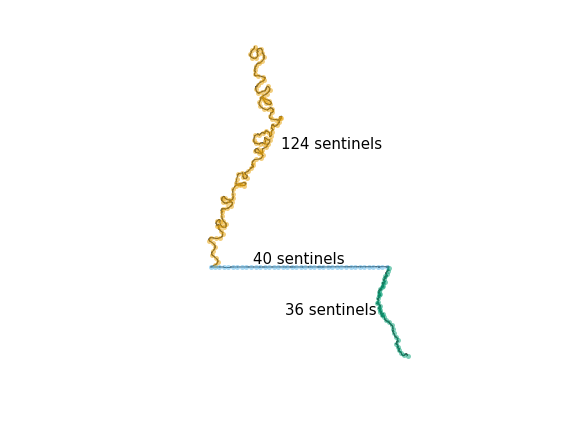
\includegraphics{figures/mississippi_counts.png}
\caption{\label{fig:mississippi_counts} Evenly spaced sentinels along the border between Mississippi and Louisiana.}
\end{figure}

Secondly, the unweighted mean treatment estimand is affected by the shape of the border between the treatment and control regions.
We illustrate this with the border separating two American States: Louisiana and Mississippi.
From North to South, the border follows the meandering Mississippi river, then takes a sharp turn to the East and becomes a straight line, until it meets the even more sinuous Pearl river, which it then follows until it reaches the Gulf of Mexico.
Sentinels placed at constant intervals along this interval will therefore be most densely packed along the Pearl River, and sparsest along the straight segment of the border (see Figure \ref{fig:mississippi_counts}).
When averaging a function over the border, those sections will therefore be overrepresented.
Troublingly, the sinuousness of the border therefore determines the estimand, and the resolution of our map can drastically change our estimate, even though the outcomes of the treatment we are studying might have nothing to do with river topographies.

Weighing the treatment effect at each sentinel location by a local density estimate would address the first issue, but not the second.
We view the unwelcome dependence of the \(\linavg\) estimand on the border topography as a side effect of ignoring the fact that the 1-dimensional treatment function \(\tau(\boundary)\) is embedded in a Euclidean 2-dimensional space.
This fact is captured by the covariance structure: sentinels in the straight segment of the border will be less strongly correlated than in the sinuous segments.
The more correlated sentinels individually carry less information about the local treatment effect.
This suggests that instead of averaging the treatment effect evenly along the border, we wish to average evenly the information contained therein.
This motivates the use of the inverse-variance weighted mean \(\invvar\), which efficiently extracts the information from the posterior to produce the weighted avereage with minimum variance.

\begin{equation}
\label{eq:invvar}
\begin{split}
    \invvar \mid Y_T, Y_C, \sigmaf, \sigman, \ell &\sim \normal\del{\mu_{\invvar \mid Y}, \Sigma_{\invvar \mid Y}} \\
    \mu_{\invvar \mid Y} &\approx \del{\ones\trans \Sigma_{\sentinels \mid Y}^{-1} \mu_{\sentinels \mid Y}} \big/ \del{\ones\trans \Sigma_{\sentinels \mid Y}^{-1} \ones}  \\
    \Sigma_{\invvar \mid Y} &\approx 1 \big/ \del{\ones\trans \Sigma_{\sentinels \mid Y}^{-1} \ones}
\end{split}\end{equation}

This estimator will automatically give more weight to sentinels in dense areas (as the variance will be lower there), and to sentinels in straight sections of the border.
While the estimand is less clear, the approach is in keeping with the philosophy of regression discontinuity designs.
We let information be our guide when averaging over our boundary, just like it guided the analysis of regression discontinuity designs to only focus on the treatment effect at the boundary.
The estimand isn't chosen by the scientist, but rather it is dictated by the limitations of the data.
    


    	\section{2GP: Testing for non-zero effect}\label{gp-testing-for-non-zero-effect}

Following the 2GP procedure, we might naturally wonder whether we can claim to have detected a significant treatment effect anywhere along the boundary.
In the hypothesis testing framework, we have two possible choices of null hypotheses.
The \textbf{sharp null} specifies that the treatment effect is zero everywhere along the boundary:
\(\tau(\boundary)=0\),
while the \textbf{weak null} only requires the average treatment effect to be zero.

\subsection{Using the inverse-variance weighted mean treatment effect posterior to test the weak null hypothesis}\label{using-the-inverse-variance-weighted-mean-treatment-effect-posterior-to-test-the-weak-null-hypothesis}

As we saw in the previous section, the ``average'' treatment effect can be defined in multiple ways.
If we choose the inverse-variance weighted mean, then \(\invvar\) has posterior given by \eqref{eq:invvar}.
While the posterior is a Bayesian object, we can use it heuristically to derive a pseudo-\(p\)-value

\begin{equation}
\begin{split}
    Z_0 &\sim \normal\del{0, \Sigma_{\invvar \mid Y}}  \\
    p^{\mathrm{INV}} &= \Pr\del{ 
        \abs{Z_0} > 
        \abs{
            \mu_{
                \invvar \mid Y
            }
        } 
    } \\
    &= 2\Phi\del{-
        \frac{
            \abs{
                \mu_{
                    \invvar \mid Y
                }
            }
        }{
            \sqrt{
                \Sigma_{\invvar \mid Y}
            }
        }
    }
\end{split}
\end{equation}

While we didn't derive this pseudo-\(p\)-value through a rigorous procedure, our simulations show that it actually has good frequentist properties.
    


    	\subsection{Likelihood-based sharp null test}\label{likelihood-based-sharp-null-test}

We can also target the sharp null hypothesis.
We first create a null model \(\modnull\),
specified as a single Gaussian process spanning the control and treatment regions,
with the same kernel and hyperparameters obtained in the 2GP procedure.
\(\modnull\) is smooth and continuous at the boundary,
and therefore accords with the sharp null hypothesis.
Intuitively, if there is a treatment effect,
the likelihood of the observations should be lower under \(\modnull\) than under \(\modalt\),
the 2\(\gp\) model as specified in equation \eqref{eq:spec2gp}.
We therefore choose the difference in log-likelihoods as our test statistic

\begin{equation}
    t = \log \Pr\del{Y_T, Y_C \mid \modalt} - \log \Pr\del{Y_T, Y_C \mid \modnull}
\end{equation}

and wish to reject the sharp null hypothesis when its observed value \(t_{obs}\) is high.

A parametric bootstrap approach is used to quantify what ``high'' means. We draw \(Y_T^*,Y_C^*\) from \(\modnull\),
using the same spatial locations as in the original data,
and then fit the two competing models to the simulated data in order to obtain the bootstrapped test statistic

\begin{equation}
    t^* = \log \Pr\del{Y_T^*, Y_C^* \mid \modalt} - \log \Pr\del{Y_T^*, Y_C^* \mid \modnull}
\end{equation}

Repeating this procedure, we obtain a distribution of \(t\) under \(\modnull\),
which we can then compare to the observed \(t\).
More precisely, we can interpret the proportion of \(t^*\) drawn above \(t_{obs}\) as a \(p\)-value.

\begin{equation}
    p^{\mathrm{lik}} = \Pr\del{t^* > t_{obs} \mid \modnull}
\end{equation}

Computationally, because the hyperparameters and locations of the units are held constant during the bootstrap, we can reuse the Cholesky decomposition of the covariance matrix, allowing the test to be performed in seconds even with hundreds of units and thousands of bootstrap samples.
    


    	\subsection{\texorpdfstring{\(\chi^2\) test for the sharp null}{\textbackslash{}chi\^{}2 test for the sharp null}}\label{chi2-test-for-the-sharp-null}

The likelihood-based sharp null above is valid and easy to understand.
But it may seem odd that the test aims to detect a non-zero treatment effect at the boundary, without any explicit reference to the boundary \(\boundary\). The test statistic and \(p\)-values can be computed without access to the sentinel positions, using only the treatment and control indicators.

To address this oddity, we can derive a test statistic directly from the posterior treatment effect along the boundary,
approximated in \eqref{eq:postvar2gp} by its mean vector \(\muvec_{\sentinels \mid Y}\)
and covariance matrix \(\Sigma_{\sentinels \mid Y}\) at the sentinel positions \(\sentinels\).
We will use \(\muvec\) and \(\Sigma\) as shorthand throughout this section.
If a \(k\)-vector \(\yvec\) has multivariate distribution \(\normal{0, \Sigma}\), then \(\yvec\trans \Sigma^{-1} \yvec\) has distribution \(\chi^2_k\).
This suggests that we could use \(S=\muvec\trans \Sigma^{-1} \muvec\) as a test statistic,
and obtain a \(p\)-value by comparing it to a \(\chi^2_k\) distribution, where \(k\) is the number of sentinels.
However, we face two problems.
Firstly, this test derived heuristically from a Bayesian posterior is invalid from a frequentist perspective.
Secondly, while \(\Sigma\) is mathematically full-rank, it is typically numerically rank-deficient.
Therefore, \(k\) overestimates the true degrees of freedom of \(\Sigma\), which invalidates the test.

Benavoli and Mangili (2015), developing a test for function equality, address the second problem by trimming the \(\Sigma\) eigenvalues \(\lambda_i\) lower than \(\epsilon \sum_{j=1}^k \lambda_j\), with \(\epsilon\) a pre-specified small number (they use 0.01).
They address the first problem by showing that the resulting \(p\)-value is conservative in certain simulation settings.
However, in our work, we found the resulting \(p\)-value to be sensitive to the arbitrarily chosen \(\epsilon\) tolerance parameter, which makes it difficult to believe its validity.

We therefore again take the parametric bootstrap approach, this time using \(S\) as the test statistic instead of the likelihood ratio.
Because \(S\) involves inverting a matrix \(\Sigma\) that is mathematically of full rank, but numerically of low rank, we may worry about the numerical stability of computing \(S\).
We rely on julia's matrix division polyalgorithm to ensure numerical stability,
and check in simulated examples that adding a small constant to the diagonal of \(\Sigma\) does not greatly affect the computed \(S\).
Furthermore, even if numerical stability was an issue,
the parametric bootstrap ensures the frequentist validity of the test,
though its power could be lowered.
    


    	\subsection{Power in simulated example}\label{power-in-simulated-example}

\begin{figure}
\centering
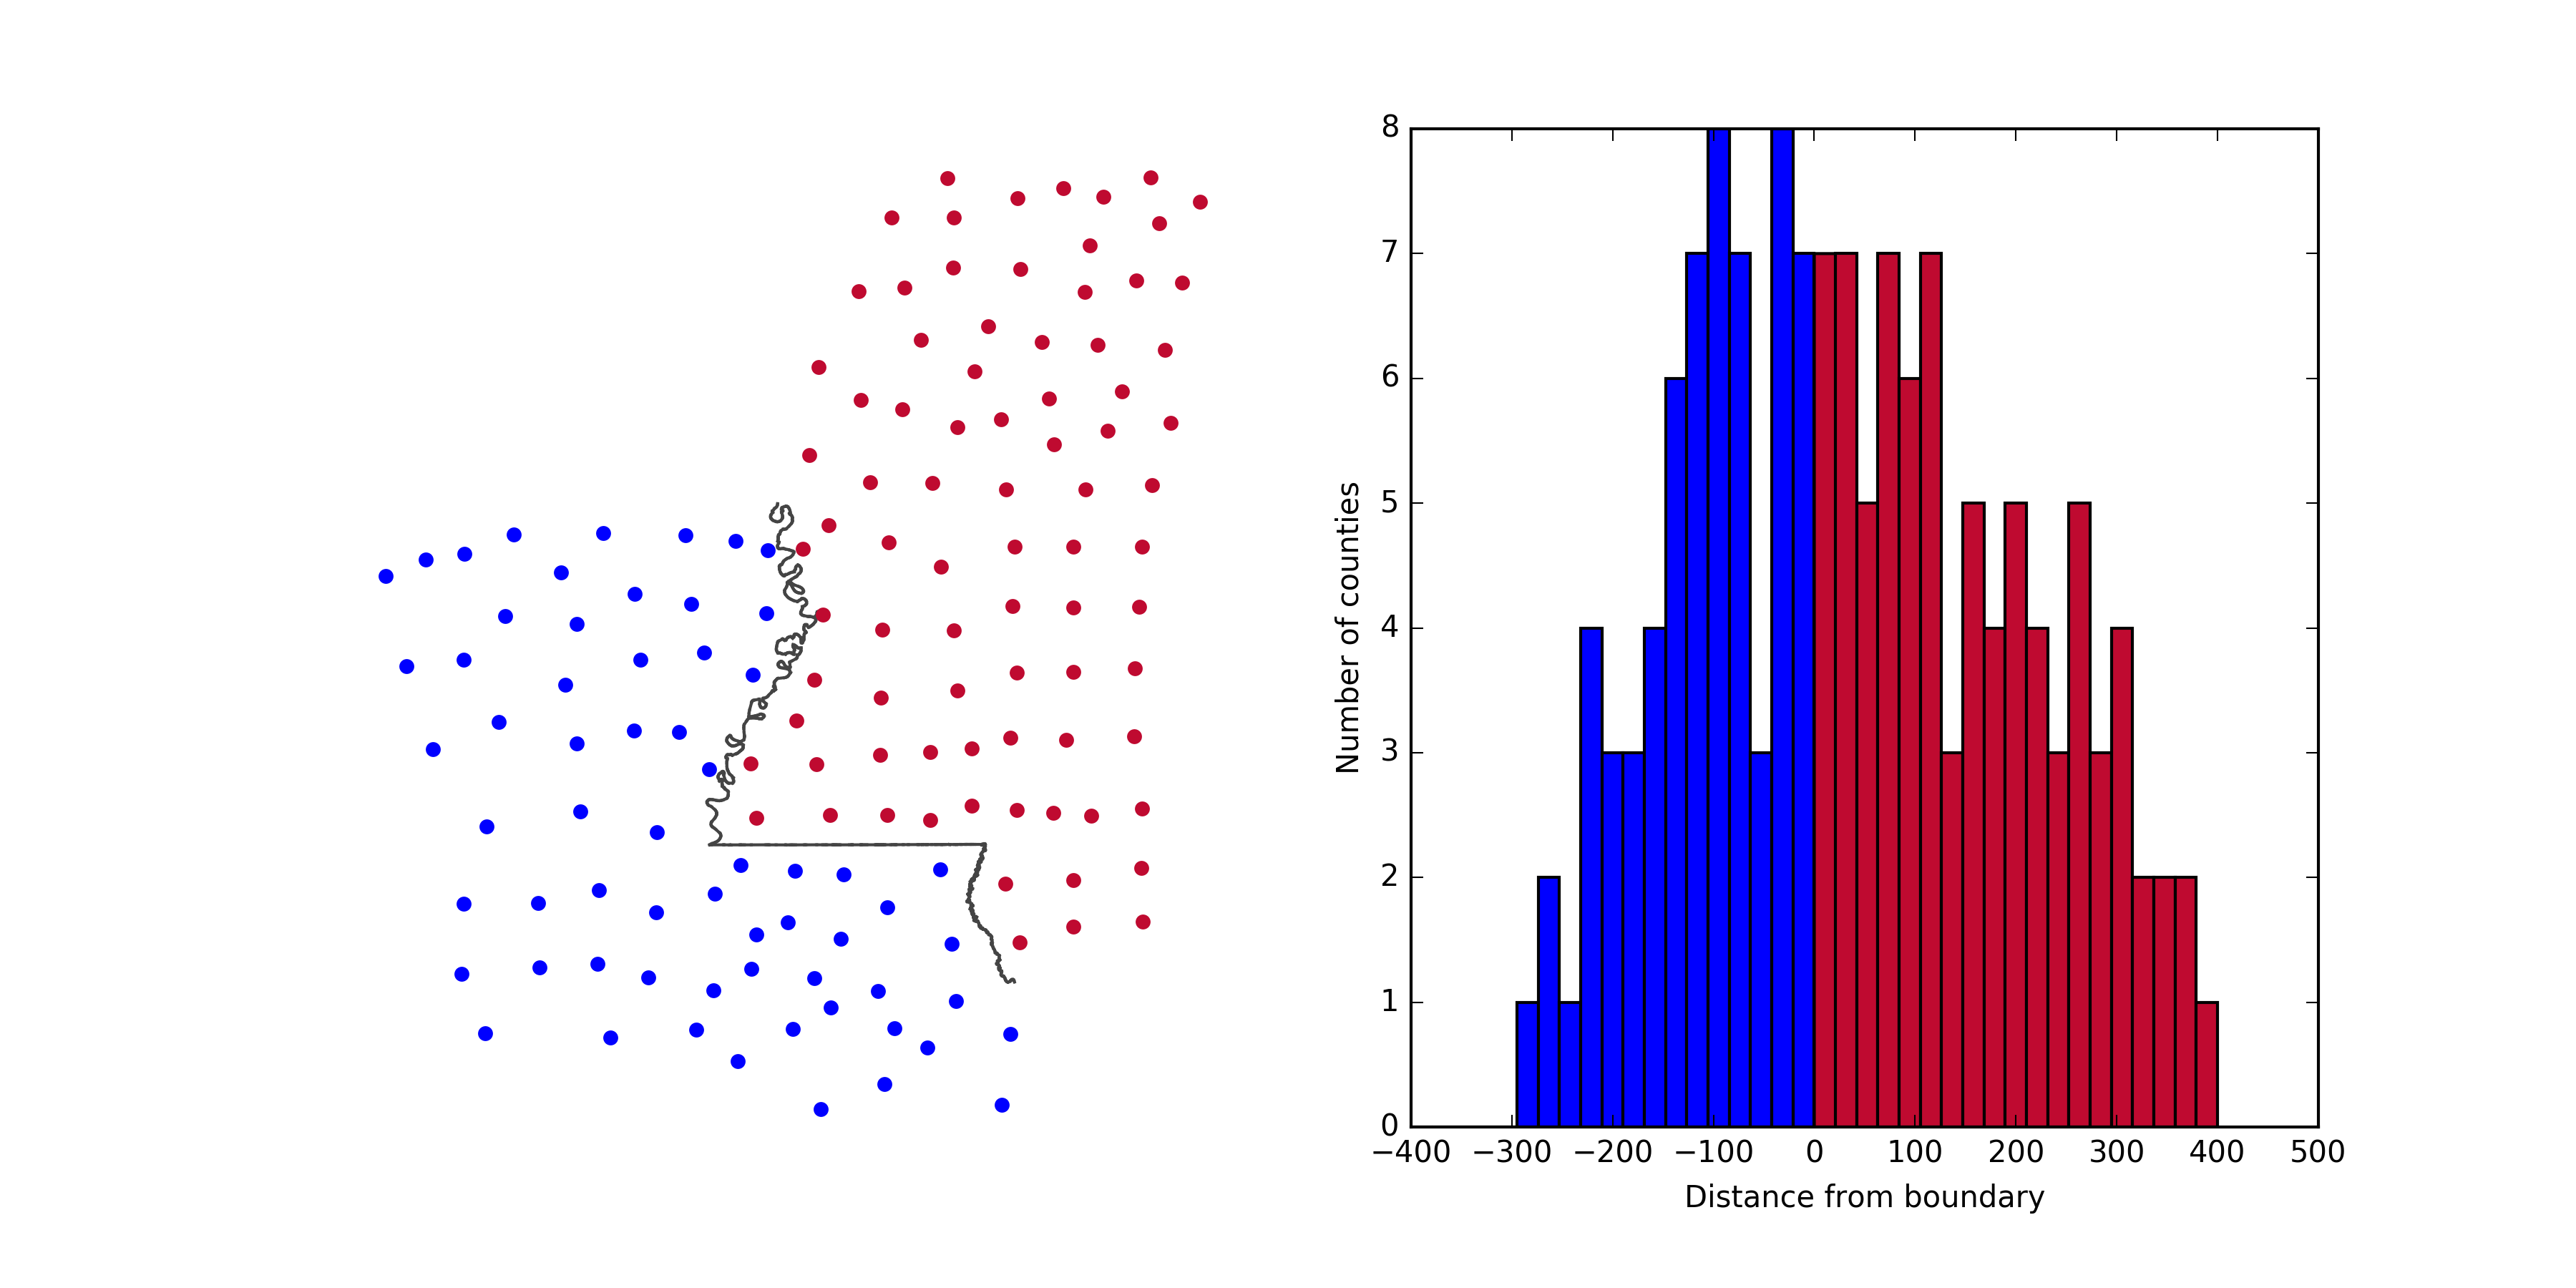
\includegraphics{figures/mississippi_counties.png}
\caption{\label{fig:mississippi_counties} Position of units in an imaginary experiment in Louisiana and Mississippi}
\end{figure}

The three tests we developed leverage different aspects of the problem, and target two different null hypotheses. One may wonder how their power compares in the presence of a treatment effect. Considering once more the boundary between Louisiana and Mississippi, we imagine an experiment where the unit of analysis is the county, located at its centroid, as shown in Figure \ref{fig:mississippi_counties}(a).
We will simulate outcomes from a single Gaussian Process covering both states. For simplicity, we fix the hyperparameters to arbitrary values: \(\sigman=\sigmaf=1.0\) and \(\ell=50\,\mathrm{km}\). We then add a constant treatment effect \(\tau\) to all the outcomes in Louisiana. The results for \(\tau=0\) (null hypothesis) and \(\tau=0.5\) are shown in Figure \ref{fig:power}.

\begin{figure}
\centering
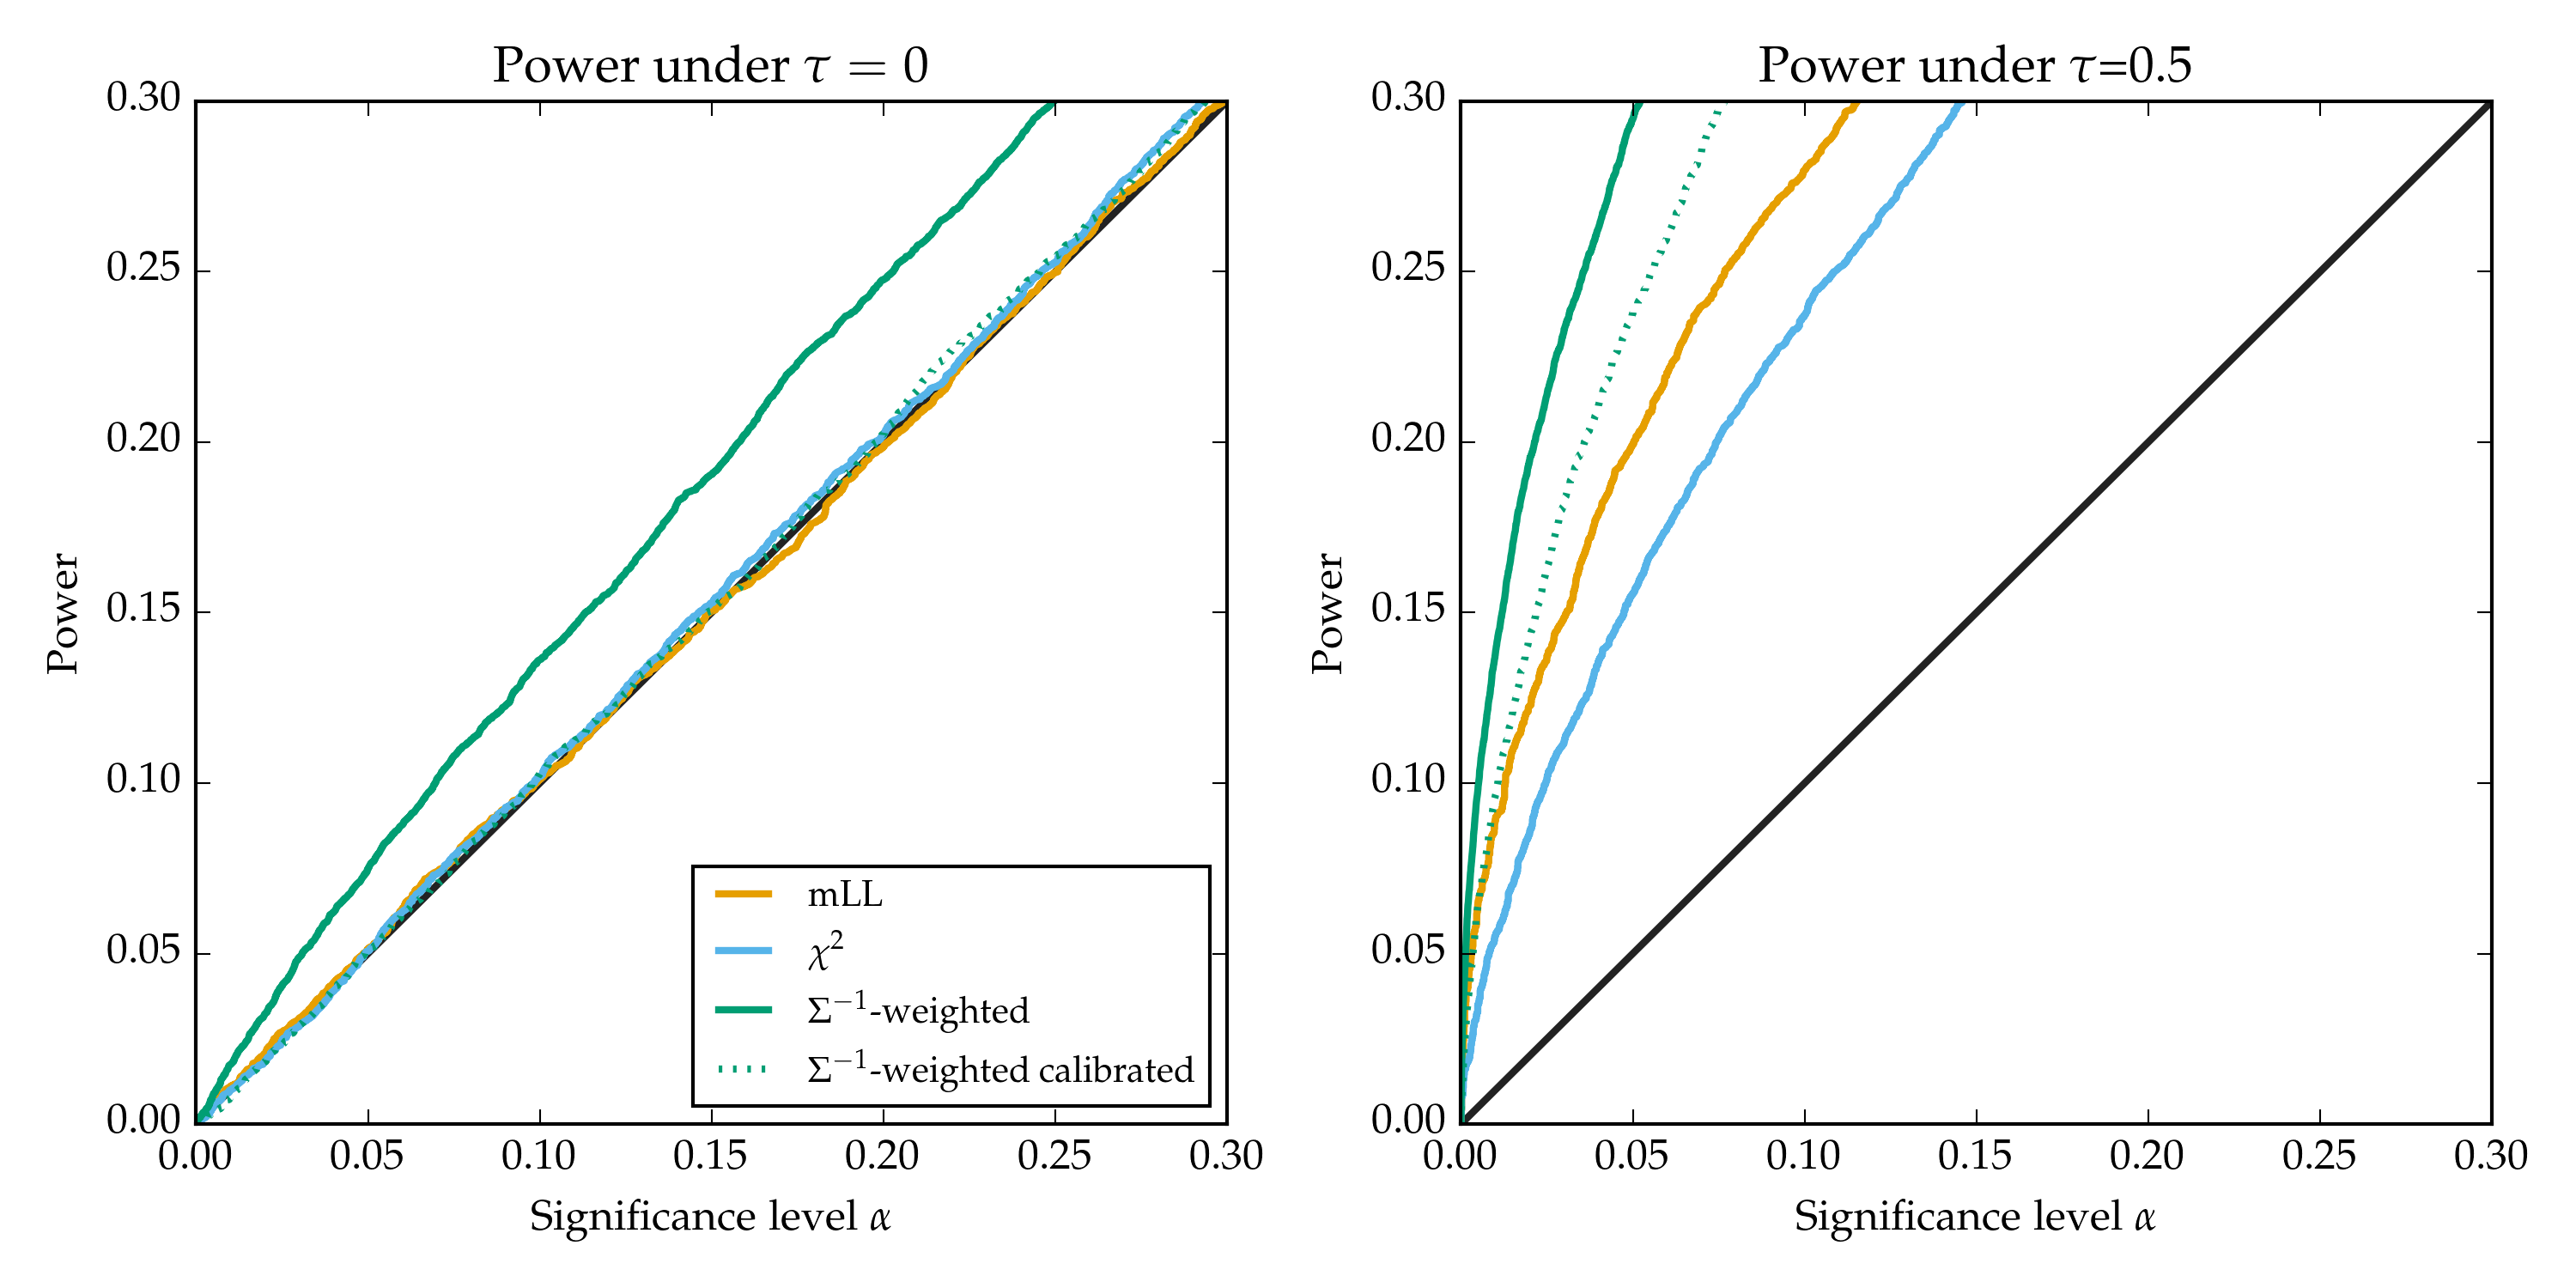
\includegraphics{figures/power_HT.png}
\caption{\label{fig:power} Power of hypothesis tests}
\end{figure}

We see that under the null, the \(p\)-values of the \(\chi^2\) and likelihood ratio tests are uniformly distributed. This is enforced by the parametric bootstrap, which draws test statistics from the same null distribution to calibrate the tests. However, the \(p\)-values for the inverse-variance test are biased down, so for example if we set \(\alpha=0.05\), we will falsely reject the null \(7.5\%\) instead of \(5\%\) of the time. While unfortunate, this is unsurprising, since the inverse-variance test was derived heuristically rather than from a rigorous frequentist procedure. It can be calibrated using the same parametric bootstrap approach that was used for the likelihood and \(\chi^2\) tests. The calibration can also be achieved analytically, since \(\mu_{\invvar \mid Y}\) is normally distributed under the null hypothesis.

Even after the calibration, the hypothesis test based on the inverse-variance mean has the highest power to detect the constant treatment effect. This can lead to a paradox: we may reject the weak null hypothesis, but fail to reject the sharp null hypothesis (using the \(\chi^2\) or likelihood test), even though rejection of the weak null should logically imply rejection of the sharp null. This paradox isn't specific to this setting, and is discussed in depth in the context of randomization-based inference by \cite{Ding:2014sf}. Therefore, in scientific contexts where the main interest is an overall (average) increase or decrease in outcomes, we recommend using the inverse-variance test to maximize power.
    


    	\subsection{Placebo tests}\label{placebo-tests}
    

\label{sec:placebo}
    	Gaussian Process models are almost always misspecified.
We do not believe that the Gaussian process with stationary squared exponential kernel is the true data-generating process, although we hope that the model is sufficiently flexible to represent reality well.
Under misspecification, we should be skeptical of results that rely on the truth of the model specification.
We therefore encourage practicioners to probe the validity of the above hypothesis tests by running a ``placebo'' test.
A placebo test repeatedly applies the hypothesis test on data that are known to have zero treatment effect (a ``placebo''),
in order to verify that the returned p-values are uniformly distributed.
In our spatial setting, we will use the treatment and control regions separately as placebo groups.
Within each placebo group, we repeatedly draw an arbitrary geographical boundary, creating new treatment and control groups.
Because the boundary was chosen arbitrarily by us, we should not expect there to be a discontinuous jump in outcomes at this boundary.
We then apply the bootstrapped likelihood test procedure described above to this arbitrarily divided data, store the results, and hope to obtain a roughly uniform distribution of p-values.
In our implementation, we drew lines that split the placebo units in half at a sequence of angles \(1\degree,2\degree,3\degree,\ldots,180\degree\).
The resulting p-values will obviously be highly correlated, so we should only expect a very roughly uniform distribution (because of the small effective sample size), but at the very least, this procedure allows us to visually verify that the p-values are not blatantly biased.
    


    	\section{Spatial advantage}\label{spatial-advantage}

Classical regression discontinuity designs often suffer from low power, requiring many units near the boundary for inference to be possible.
In the spatial RDD setting, we might worry that the situation is worse, as geographical datasets with many units packed along the boundary are uncommon.
In geographical settings, each unit (e.g.~household or counties) normally takes up space, so there is a limit to how densely packed units can be near the boundary.
And boundaries often include sparsely populated segments, e.g.~running through parks, industrial areas, or farmland.
The intuition that spatial RDDs will therefore suffer from low power is correct, inasmuch as at any given point along the boundary, the posterior variance of \(\tau(\boundary)\) will typically be high.
But once we pool the information into an average treatment effect, or perform a sharp test, spatial RDDs can be more powerful than classical RDDs, with the same number of units at the same distance from the boundary.

We illustrate this statement once more with the Louisiana-Mississippi example.
The variance of the inverse-variance weighted treatment effect \(\invvar\) is thence only a function of the positions of the units, available analytically by plugging the posterior variance \eqref{eq:postvar2gp} into the inverse-variance estimator \eqref{eq:invvar}.
Following this procedure, we obtain a posterior standard deviation of the average treatment effect of 0.31.
We then create a one-dimensional regression discontinuity design for the same setting, by using each unit's distance from the boundary as the covariate \(x\), the distribution of which is shown in Figure \ref{fig:mississippi_counties}(b).
Following the exact same 2GP procedure with the same hyperparameters as in the spatial setting, and with a discontinuity at \(x=0\), we again compute the posterior standard deviation of the treatment effect at the boundary (now a single number rather than a continuous function) , this time obtaining 0.58.
This higher figure indicates that, perhaps counter-intuitively, the spatial experiment actually has more power than its one-dimensional analog.

To gain intuition about the higher power of the spatial RDD, we turn to the interpretation of regression discontinuity designs as natural experiments {[}need reference{]}.
Near the discontinuity, we can reasonably claim that the side of the discontinuity that each unit fell into was largely dictated by random noise in the covariate.
This in turn allows us to claim that a natural randomized experiment took place near the boundary, with treatment and control units coming from the same population.
We can extend this interpretation to the spatial setting, by conceiving of multiple correlated experiments taking place all along the boundary.
The average treatment effect estimator then pools the information supplied by all of these experiments.
The question then becomes: do we get more powerful inference by grouping all the units into a single experiment, or by spreading them along a multitude of weaker experiments?
There are two sources of uncertainty in our model: the observation noise \(\epsilon_i\), and the underlying processes \(g_T\) and \(g_C\). Adding more units to a single experiment allows us to cancel out more of the observation noise, but if the new units aren't added closer to the discontinuity, uncertainty always remains in \(g_T\) and \(g_C\). In the spatial setting, however, we observe multiple realizations of the Gaussian process, and therefore do not suffer from the same diminishing returns.
    


    	\section{Example: NYC school districts}\label{example-nyc-school-districts}

We illustrate the analysis of geographical regression discontinuity designs using house sales data from New York City.
The city publishes information pertaining to property sales within the city in the last twelve months on a rolling basis.
This includes the sale price, building class, and the address of the property.
Public schools in the city are all part of the City School District of the City of New York, but the city-wide district is itself divided into 32 sub-districts.
Within these districts, schools also have attendance zones, and children living within a zone are guaranteed attendance in their zone school unless the school is full {[}is this true? \href{http://insideschools.org/elementary/how-to-apply}{insideschools.com gives a more complete picture}{]}.
It is commonly held {[}could cite \href{https://www.cityrealty.com/nyc/market-insight/features/trending-in-ny/buying-renting-school-zone-district-what-you-need-know/3661}{this article at cityrealty.com}{]} that school districts therefore have an impact on real estate price, as parents are willing to pay more to live in districts with better schools.
We therefore ask: can we measure a discontinuous jump in house prices across school district boundaries?
    


    	\subsection{Preprocessing}\label{preprocessing}

In order to model the property sale prices with a stationary Gaussian process, we need to obtain their location on a Euclidean grid. We geocode the address of each sale by merging the sales with NYC's Pluto database, which contains X and Y coordinates for each house, identified by its borough, zip code, block and lot. These coordinates are given in the \texttt{EPSG:2263} projection in units of feet. We use this projection throughout this example. For addresses that do not find a match in Pluto, we use google's geocoding API to obtain a latitude and longitude, which we then project to \texttt{EPSG:2263}.

We then filter the sales data as follows, by removing
1. sales of properties without a reported sale price
1. sales of properties outside of the residential building class categories (``one family dwellings'', ``two family dwellings'', ``three family dwellings'', ``tax class 1 condos'', ``coops - walkup apartments'', ``coops - elevator apartments'', ``condos - walkup apartments'', ``condos - elevator apartments'', ``condos - 2-10 unit residential'', ``condo coops''),
2. any sale with missing data in the sale price, square footage, property covariates, geographical coordinates (due to failed geocoding),
3. sales outside of any NYC school district,
4. properties smaller than 100 sq ft, and
5. outliers in the price per square foot.
    


    	\subsection{Exploratory analysis}\label{exploratory-analysis}

\begin{figure}
\centering
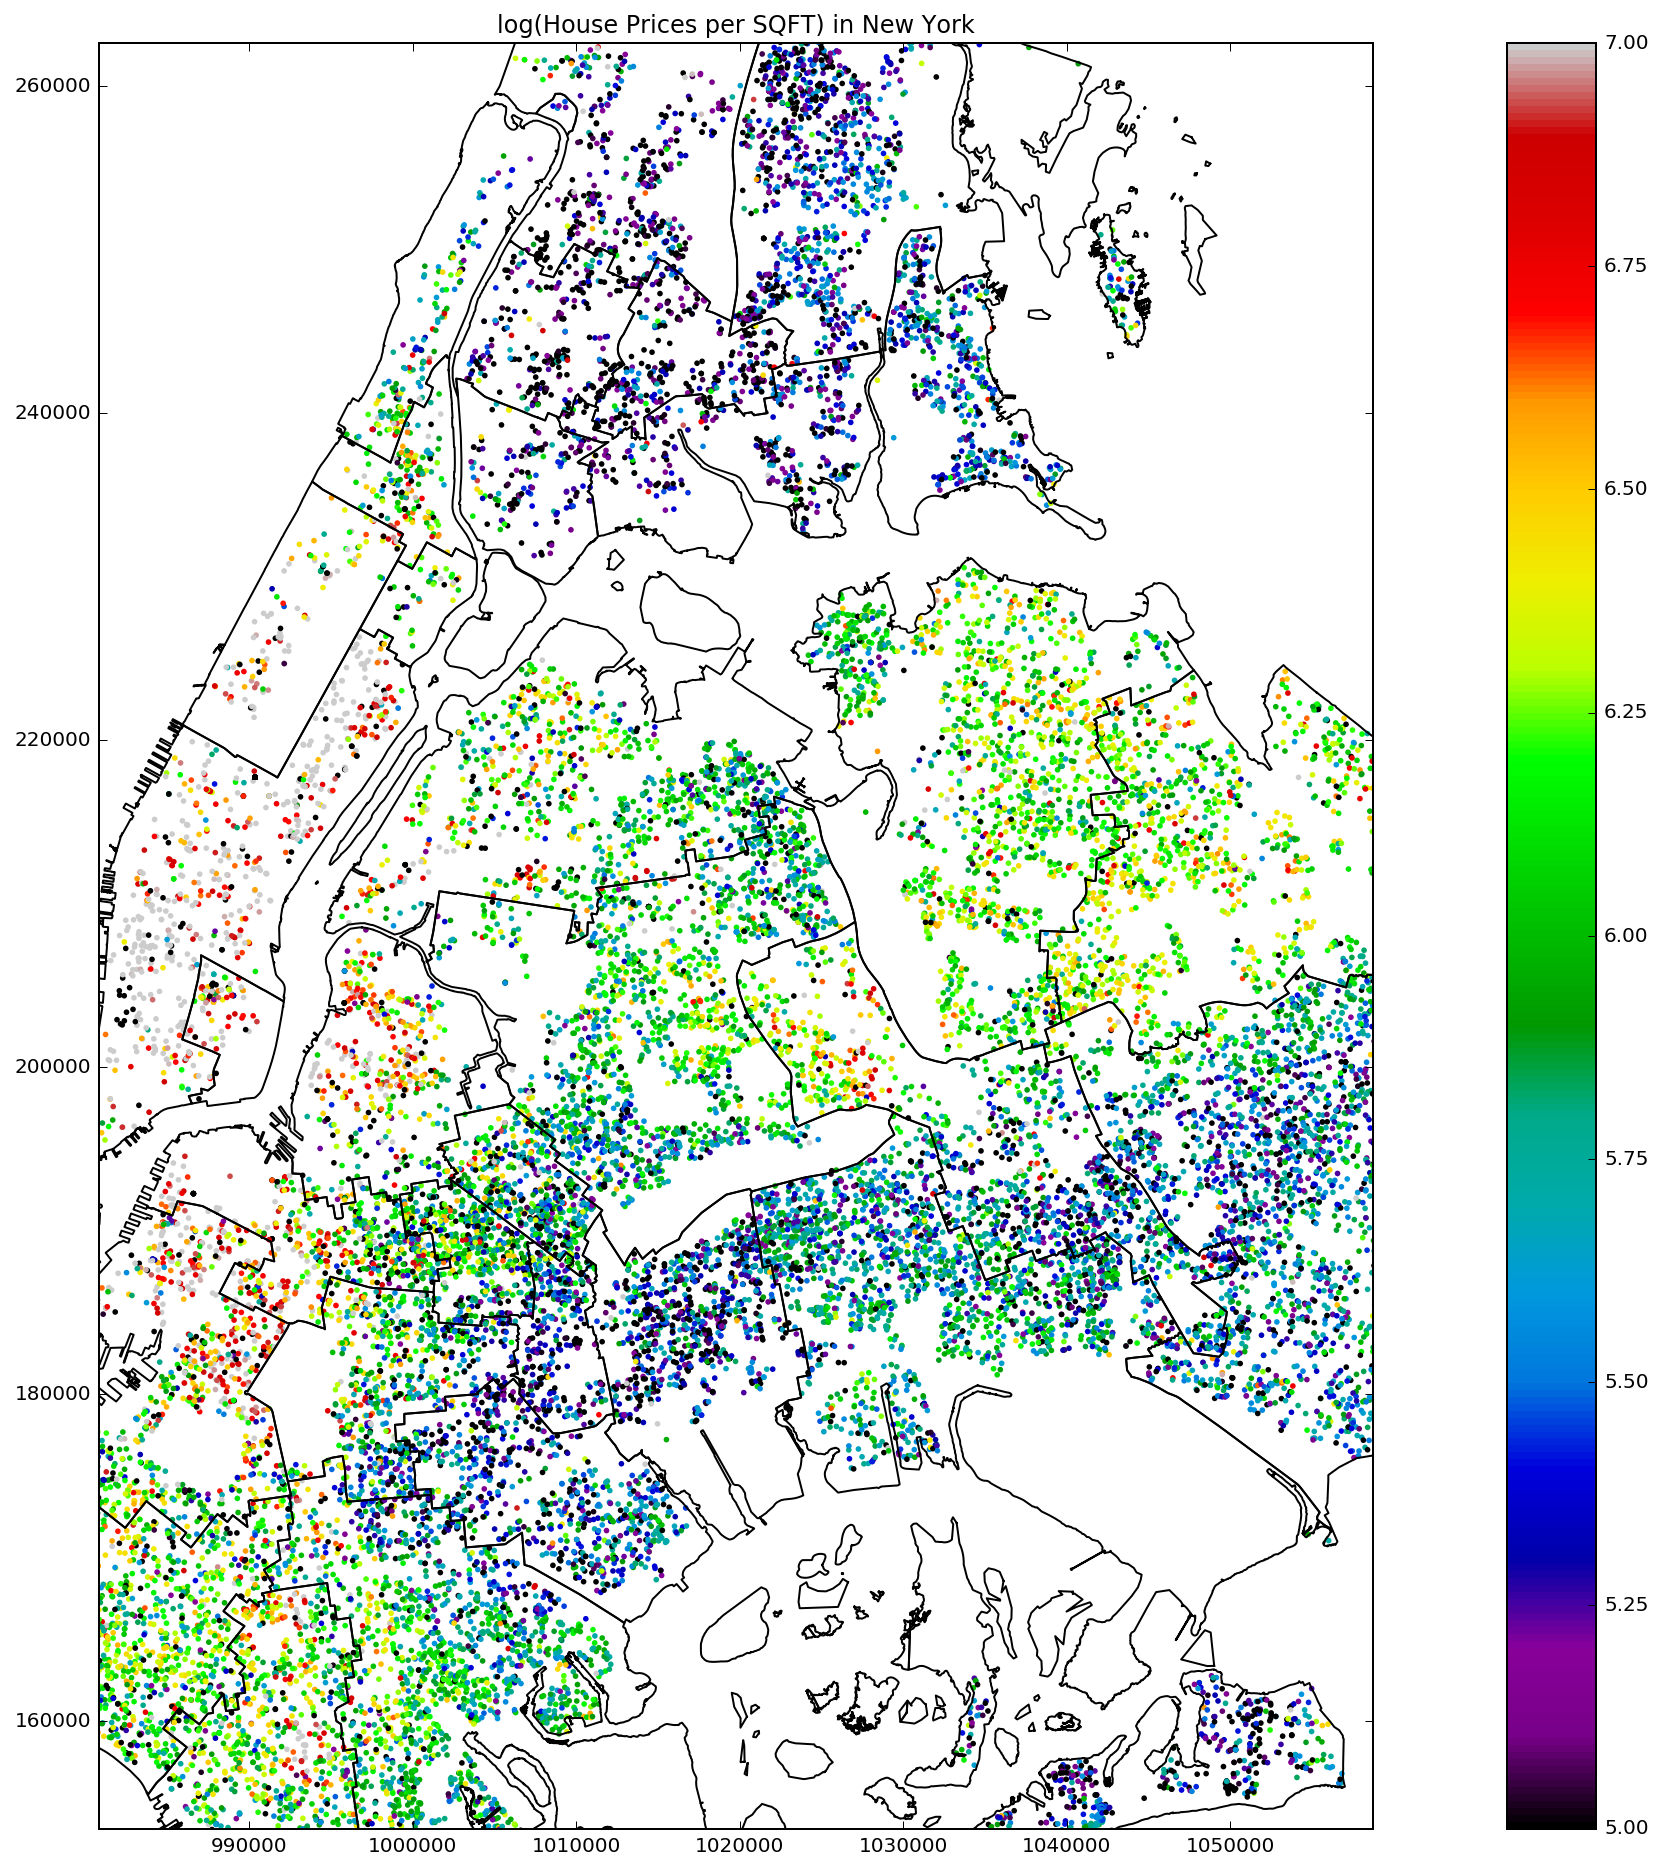
\includegraphics{NYC/NYC_plots/NYC_sales.png}
\caption{sales map}
\end{figure}
    


    	\subsection{Model for property prices}\label{model-for-property-prices}

The outcome of interest is price per square foot. As is often done in the real estate literature, we take its logarithm to reduce the skew of the outcome. The complete model is then a Gaussian Process over the geographical covariates \(\svec\) super-imposed with a linear regression on the property covariates (building and tax class). Within a school district we could write the model as {[}suggestions for clearer notation welcome{]}:

\begin{equation}
\begin{split}
    Y_i &= \log\del{ \frac{\saleprice_i}{\sqft_i}} =
        \begin{split}
             \mu_{\district\sbr{i}} + \beta_{1,\tax\sbr{i}} + \beta_{2,\building\sbr{i}} \\
                  + f_{\district\sbr{i}}(\svec_i) + \epsilon_i \\
         \end{split}
    \\
    \epsilon_i &\sim \normal\del{0, \sigma_y^2} \\
    \mu_{j} &\sim \normal\del{\bar{Y}_j, \sigma_\mu^2} \\
    \beta_{1j},\beta_{2j} &\sim \normal\del{0, \sigma_\beta^2} \\
    f_j(\svec_i) &\sim \gp\del{0, k(\svec, \svec')} \\
    k(\svec, \svec') &= \sigmaf^2 \exp\cbr{ - \frac{(\svec-\svec')\trans(\svec-\svec')}{2\ell^2}}
\end{split}
\end{equation}

A visual inspection of the house sales map above suggests examining the boundary between districts 19 and 27. Importantly, the boundary between the two districts is also part of the boundary between Brooklyn and Queens, so we won't be able to attribute a causal effect solely to the difference in school districts. We are first and foremost \emph{measuring} a discontinuity in the house prices at the district. Attributing the discontinuity to a particular cause (school district or borough) is an interpretation that is not directly supported by the data.
A histogram of \(Y\) in both districts also shows that marginally the house prices are very different.
Our goal is to establish that this difference is measurable at the boundary, and not merely an underlying trend that spans both districts.

\begin{figure}
\centering
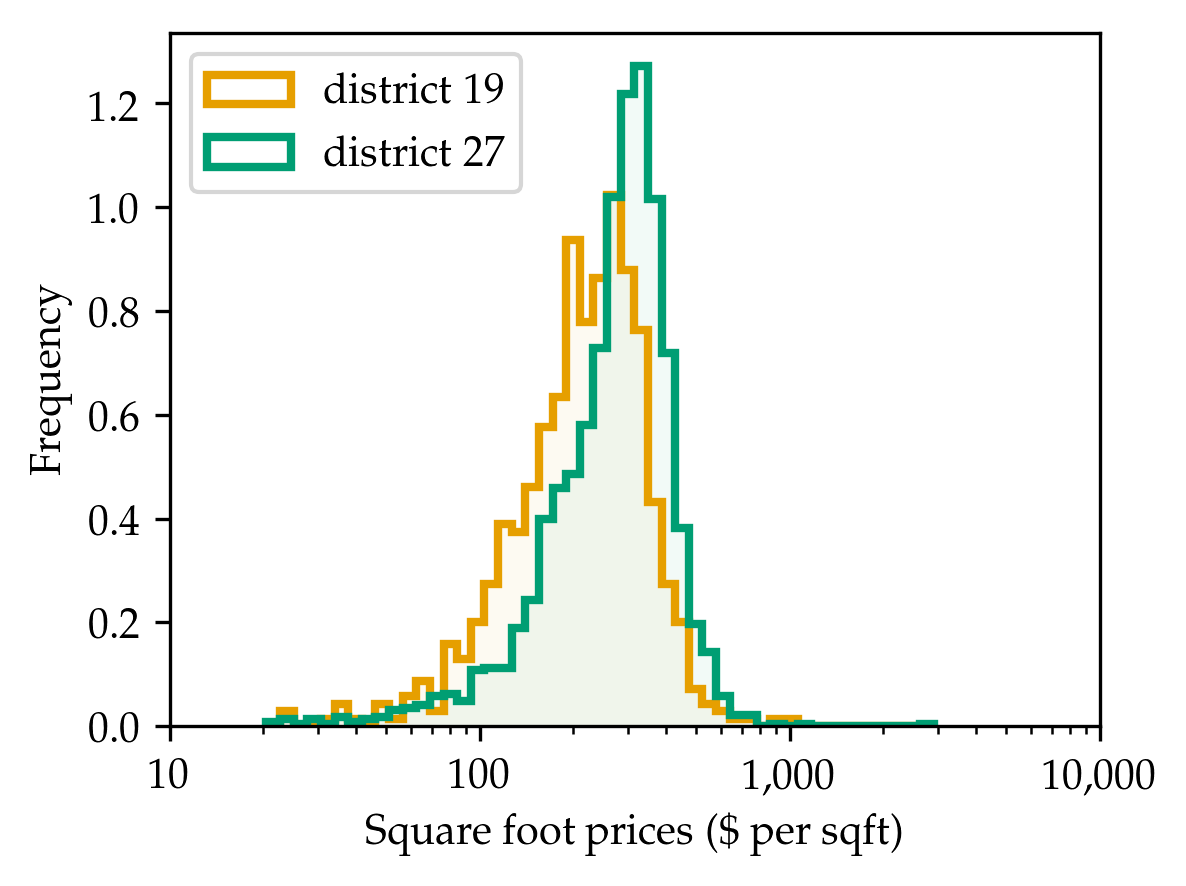
\includegraphics{NYC/NYC_plots/sales_histogram_19-27.png}
\caption{}
\end{figure}
    


    	\subsection{parameter optimization}\label{parameter-optimization}

We initially fit the hyperparameters \(\sigma_\beta\), \(\sigmaf\), \(\ell\) and \(\sigman\) by optimizing the marginal log-likelihood of the data within a single district. We choose district 27 as it contains more sales. We hold \(\sigma_\mu\) fixed to 10 to give the district means \(\mu_j\) a fairly uninformative prior. The fitted hyperparameters were \(\sigman=0.4179\), \(\sigmaf=0.2426\), \(\sigma_\beta=0.1306\), and \(\ell=3378.5800~\text{ft}\).
    


    	\subsection{cliff face}\label{cliff-face}

We seek the treatment effect function \(\tau(\boundary)\) between the two districts. We could proceed by computing the joint predictive distributions \(g_T(\sentinels),g_C(\sentinels) \mid Y_T, Y_C, \sigma_\beta,\sigmaf,\ell,\sigman\), which is a \(2 n_{\sentinels}\)-dimensional multivariate normal distribution. Instead, we obtain the posterior means of the \(\beta_{1j}\) and \(\beta_{2j}\) coefficients, extract the residuals \(Y_T-D_T \hat{\beta}\) and \(Y_C-D_C \hat{\beta}\). This decorrelates \(g_T(\sentinels)\) and \(g_C(\sentinels)\) so they become independent multivariate normal distributions \(g_T(\sentinels) \mid Y_T, \hat\beta, \sigmaf,\ell,\sigman\) and \(g_C(\sentinels) \mid Y_C, \hat\beta, \sigmaf,\ell,\sigman\). In this example, we find that the posterior variance of \(\beta\) is low, and therefore the two approaches yield very similar results, but conditioning on the estimate of \(\beta\) is computationally convenient. We therefore proceed with this two-step approach.

Equipped with multivariate normal posteriors on \(g_C(\sentinels)\) and \(g_T(\sentinels)\), which are uncorrelated conditional on \(\beta=\hat\beta\), we can now take their difference according to the procedure outline in section \ref{sec:twogp}, to obtain the posterior distribution of the cliff-face \(\tau(\sentinels)\) obtained at the sentinel locations.
The cliff-face is shown in Figure~XX, and shows that the estimated \(\tau(\sentinels)\) is negative everywhere along the border, which corresponds to higher property prices in district 27.
However, the credible envelope is wide, especially in the Southern section of the border, and therefore it isn't clear that this effect isn't due to random variation.

The treatment effect can also be visualized directly in Figure~XX as the difference between the two log-price mean surfaces \(g(\svec)\). This pictures also gives a better sense of the important spatial variation in prices captured by the model, which explains the wide credible envelope in the cliff face, despite the large number of sales in both districts.
    


    	\begin{figure}
\centering
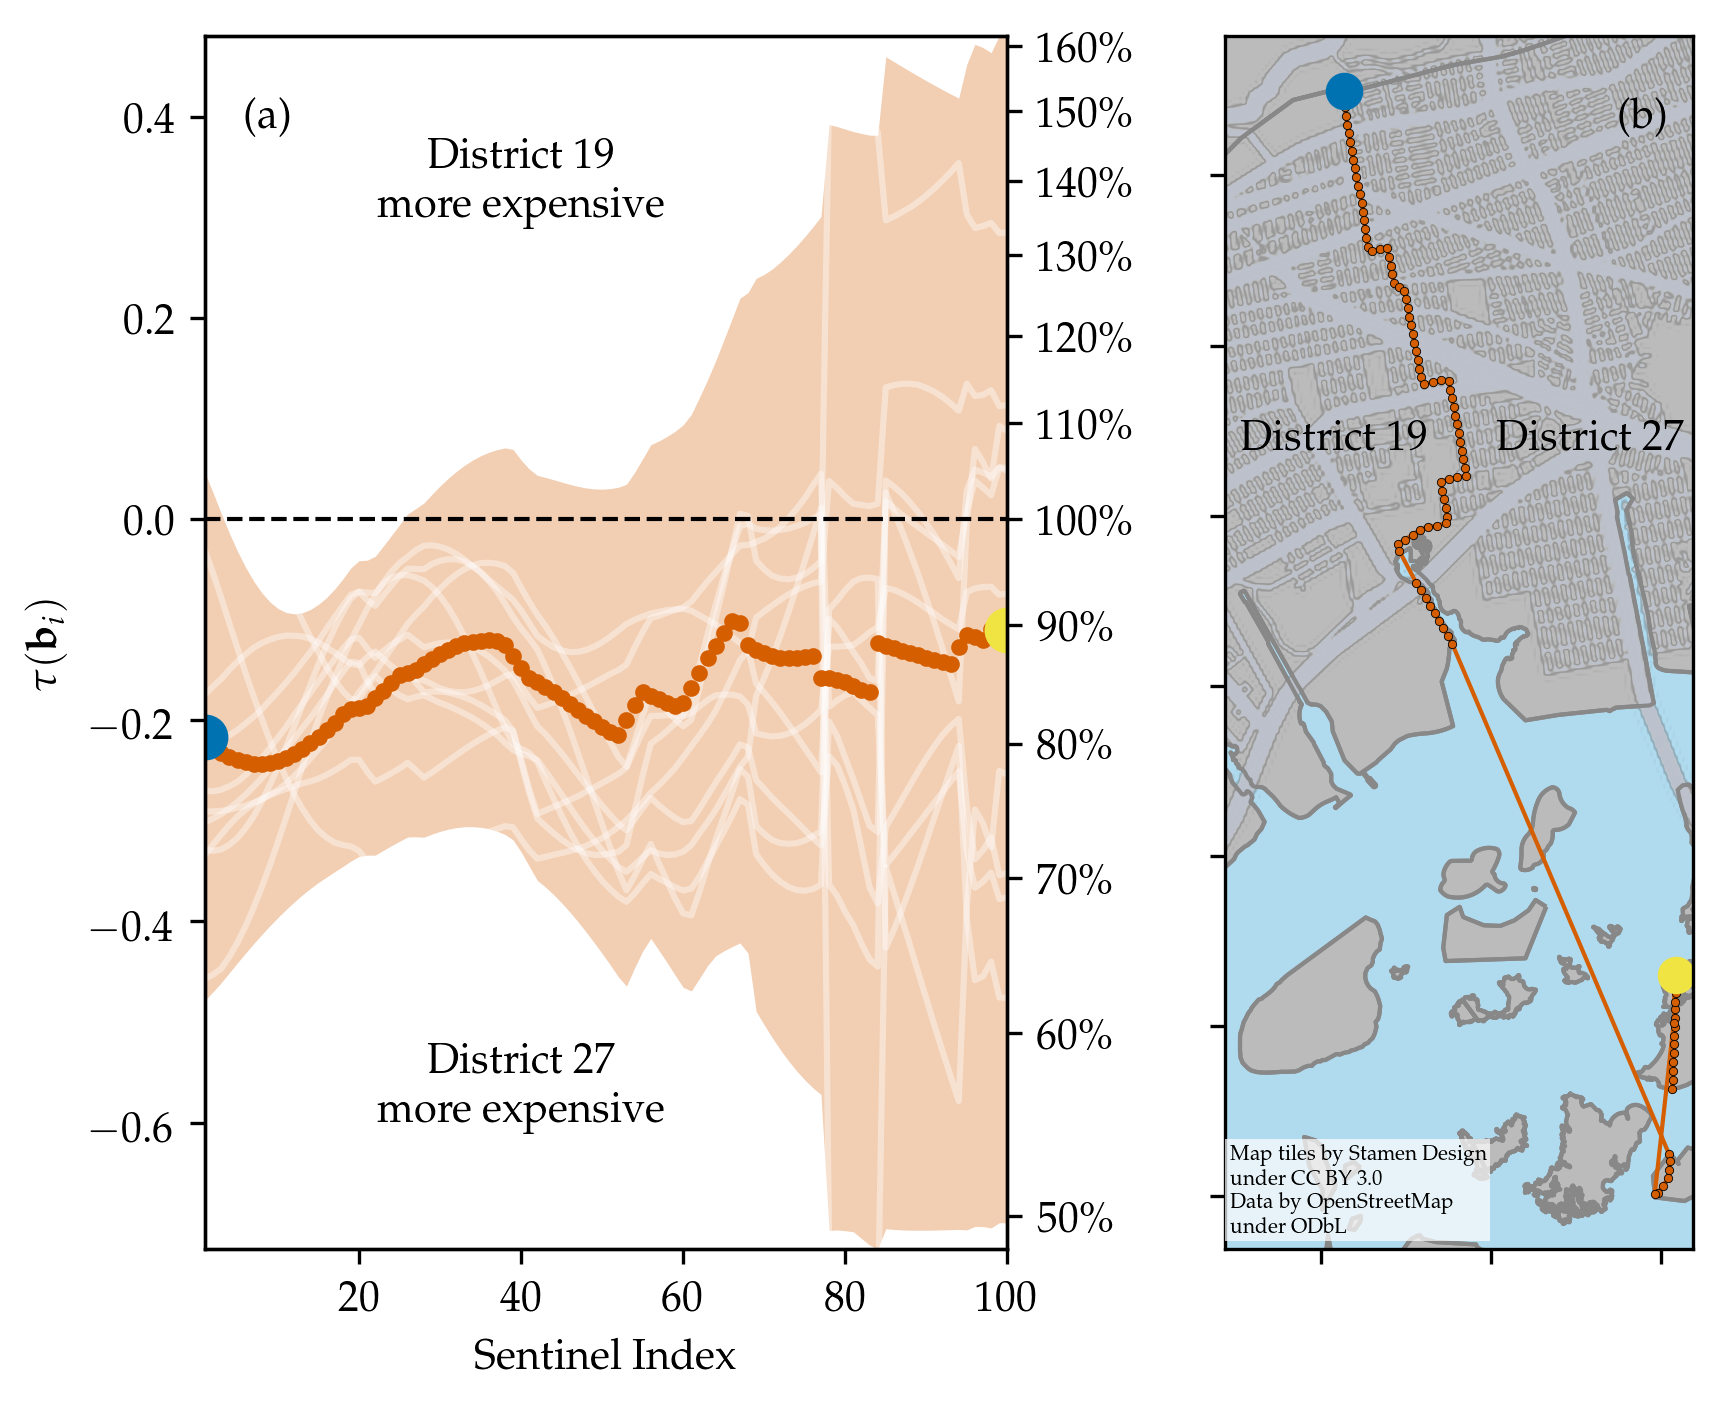
\includegraphics{NYC/NYC_plots/NYC_cliff_face.png}
\caption{NYC cliff face}
\end{figure}
    


    	\begin{figure}
\centering
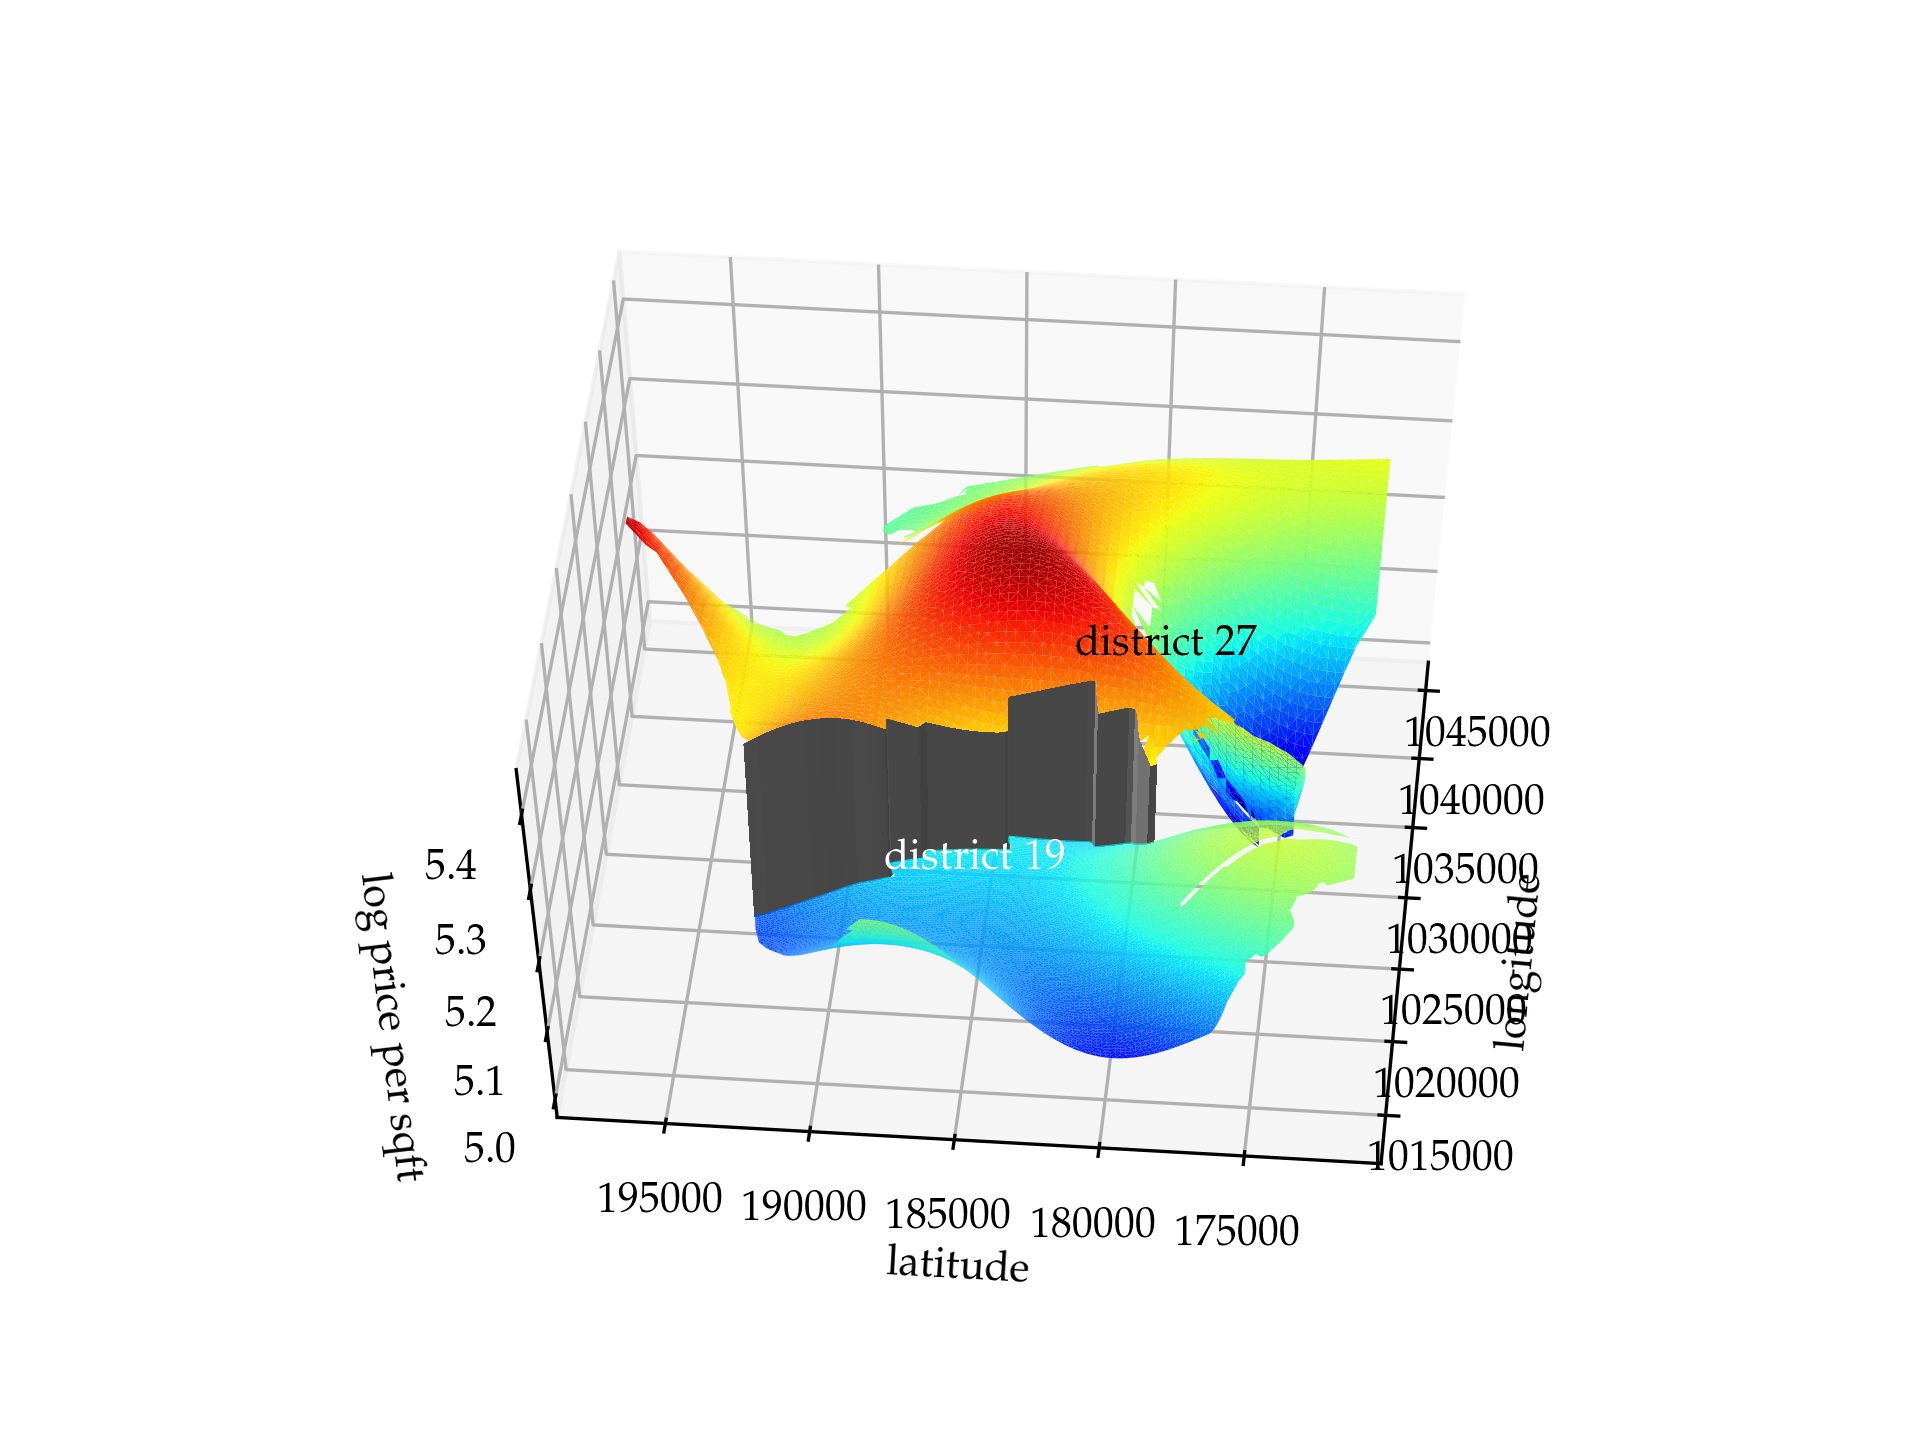
\includegraphics{NYC/NYC_plots/NYC_surface_plot_multi.png}
\caption{NYC surface plot}
\end{figure}
    


    	\subsection{Average Log-Price Increase}\label{average-log-price-increase}

The cliff-face plot shows a negative treatment effect everywhere along the border, which can be averaged by the estimators we developed in section~XX. The most obvious approach is to take an unweighted mean at each equispaced sentinel, which has posterior distribution

\begin{equation}
\begin{split}
    \linavg \mid Y_T, Y_C, \sigmaf, \sigman, \hat{\beta}, \ell &\sim \normal\del{-0.198, 0.091^2}\,\text{and tail probability} \\
    \Pr\del{\linavg > 0 \mid Y_T, Y_C, \sigmaf, \sigman, \hat{\beta}, \ell} &= 1.515\% \,.
\end{split}
\end{equation}

The inverse-variance weighted mean estimator is robust to changes in the border topology, and gives higher weight to sections of the border where the difference in house prices is easier to measure. It is guaranteed to minimize the posterior variance amongst weighted mean estimators, which is reflected here by the narrower posterior distribution

\begin{equation}
\begin{split}
    \invvar \mid Y_T, Y_C, \sigmaf, \sigman, \hat{\beta}, \ell &\sim \normal\del{-0.192, 0.059^2}\,\text{and reduced tail probability} \\
    \Pr\del{\invvar > 0 \mid Y_T, Y_C, \sigmaf, \sigman, \hat{\beta}, \ell} &= 0.017\% \,.
\end{split}
\end{equation}

This estimate corresponds to a 21\% increase in price per square foot from district 19 to district 27.
    


    	\subsection{Significant Difference in Price?}\label{significant-difference-in-price}

The inverse-variance weighted mean treatment effect hints at a significant treatment effect.
But the posterior tail probability cannot be interpreted as a \(p\)-value.
For this, we turn to the three tests developed in section~XX.
In applied settings, running multiple tests invalidates their results,
but as we are proposing this new methodology,
we apply all three tests in order to gain insight into their differences.
Their results are found in Table~XX.

\begin{longtable}[]{@{}ll@{}}
\toprule
Test & \(p\)-value\tabularnewline
\midrule
\endhead
\(\chi^2\) bootstrap & 0.145\tabularnewline
mLL bootstrap & 0.0015\tabularnewline
\(\invvar\) uncalibrated & 0.0003\tabularnewline
\(\invvar\) calibrated & 0.0005\tabularnewline
\bottomrule
\end{longtable}

The three tests tell very different stories.
The \(\chi^2\) test fails to reject the null hypothesis even at the \(\alpha=0.1\) level.
This strongly contradicts the inverse-variance test and its low \(p\)-value of \(0.0005\),
backed by the likelihood-ratio test with \(p=0.0015\).
The possibility of such a contradiction was anticipated in section~XX, where we saw that the \(\chi^2\) has the lowest power of the three tests, and therefore could easily fail to reject an effect that is easily detected by the inverse-variance test.
Because the inverse-variance test has the highest power in detecting constant treatment effects, we would recommend its use in applications ---~such as this one~--- where a very heterogenous treatment effect is not expected.
    


    	\subsubsection{placebo tests}\label{placebo-tests}

To assess the validity of the three tests, we apply the placebo tests that we devised in Section~X.
Within each district, we split the data in half by a line at angles \(1\degree,3\degree,5\degree,6\degree,\ldots,179\degree\).
Because these lines were drawn arbitrarily, we don't expect a discontinuous treatment effect between the two halves, and so we hope to see a uniform distribution of placebo \(p\)-values.
However, these tests will be highly correlated,
and so the low effective sample size could lead to some apparent departures from uniformity.
There is in fact visible autocorrelation in the graphs of placebo \(p\)-values as a function of angle.

\begin{figure}
\centering
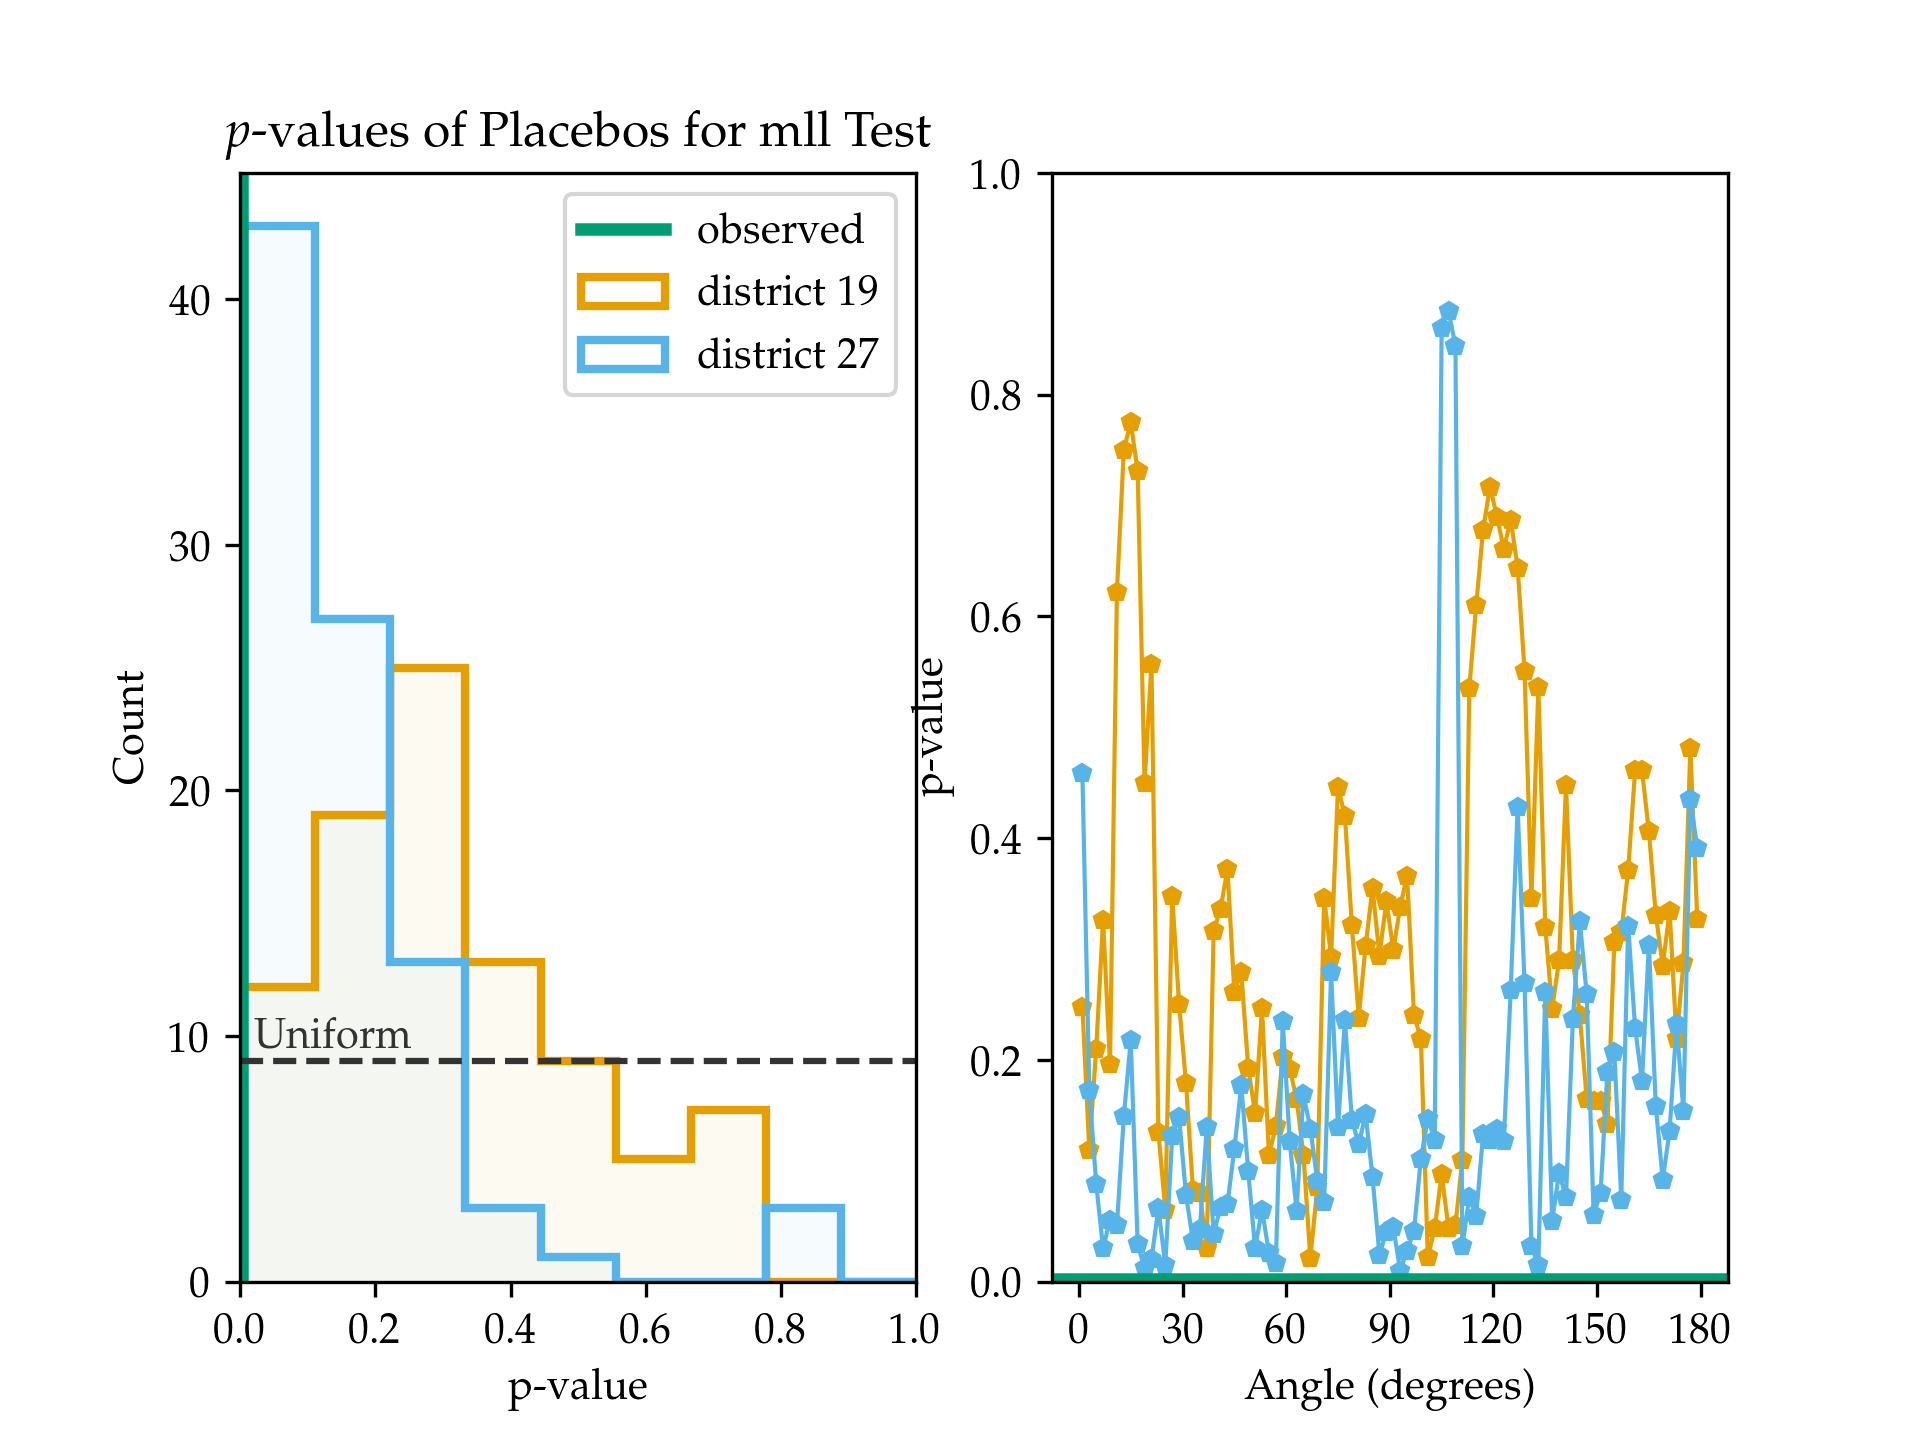
\includegraphics{NYC/NYC_plots/placebo_mLL.png}
\caption{Placebo test for mLL test}
\end{figure}

\begin{figure}
\centering
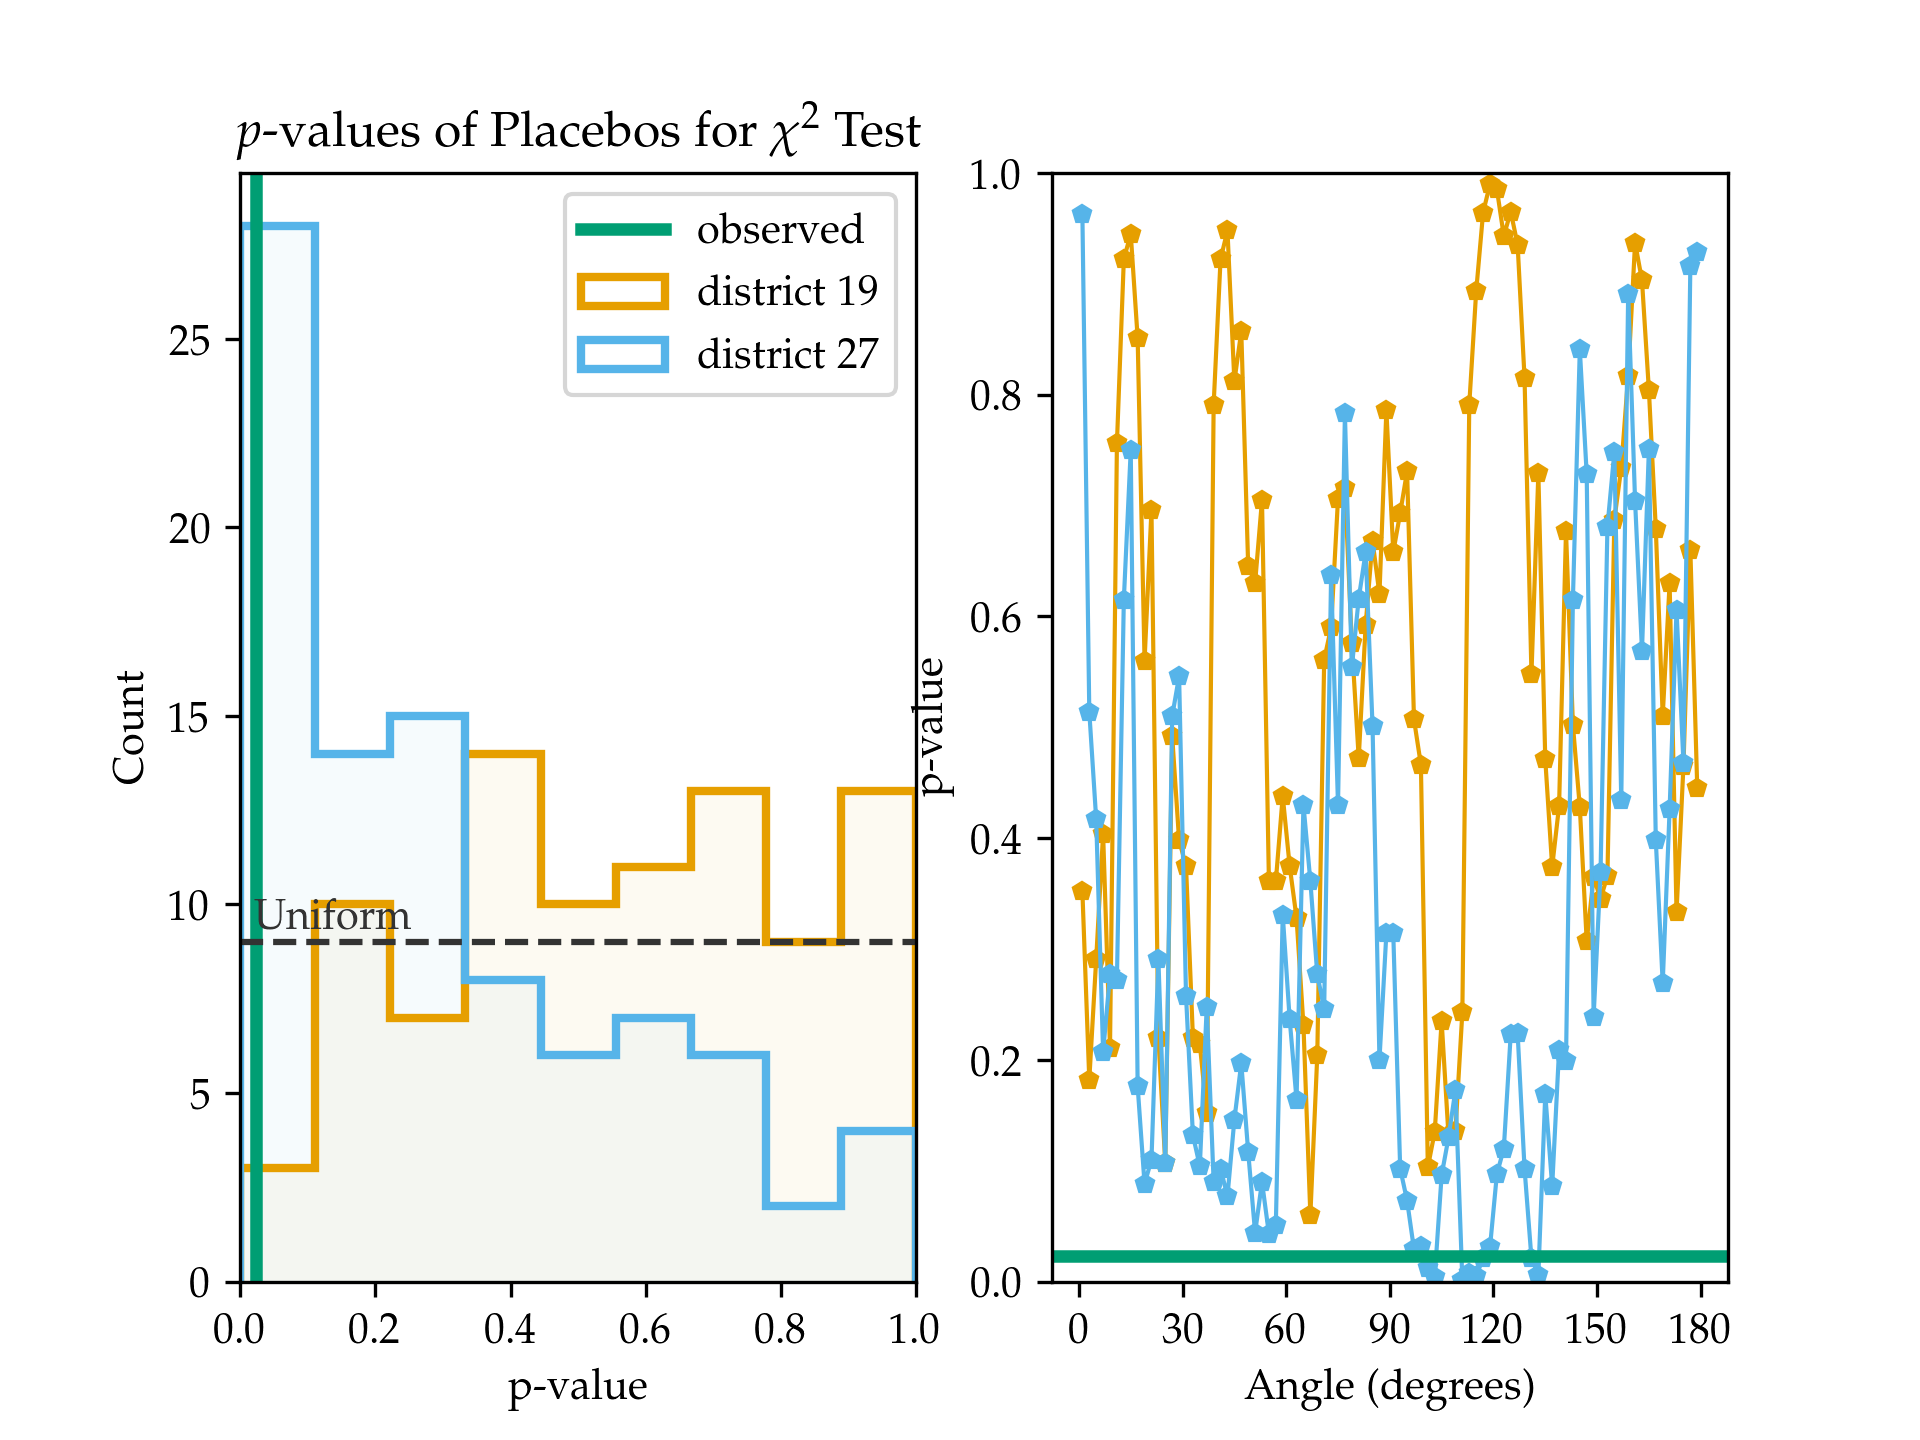
\includegraphics{NYC/NYC_plots/placebo_chi.png}
\caption{Placebo test for \(\chi^2\) test}
\end{figure}

\begin{figure}
\centering
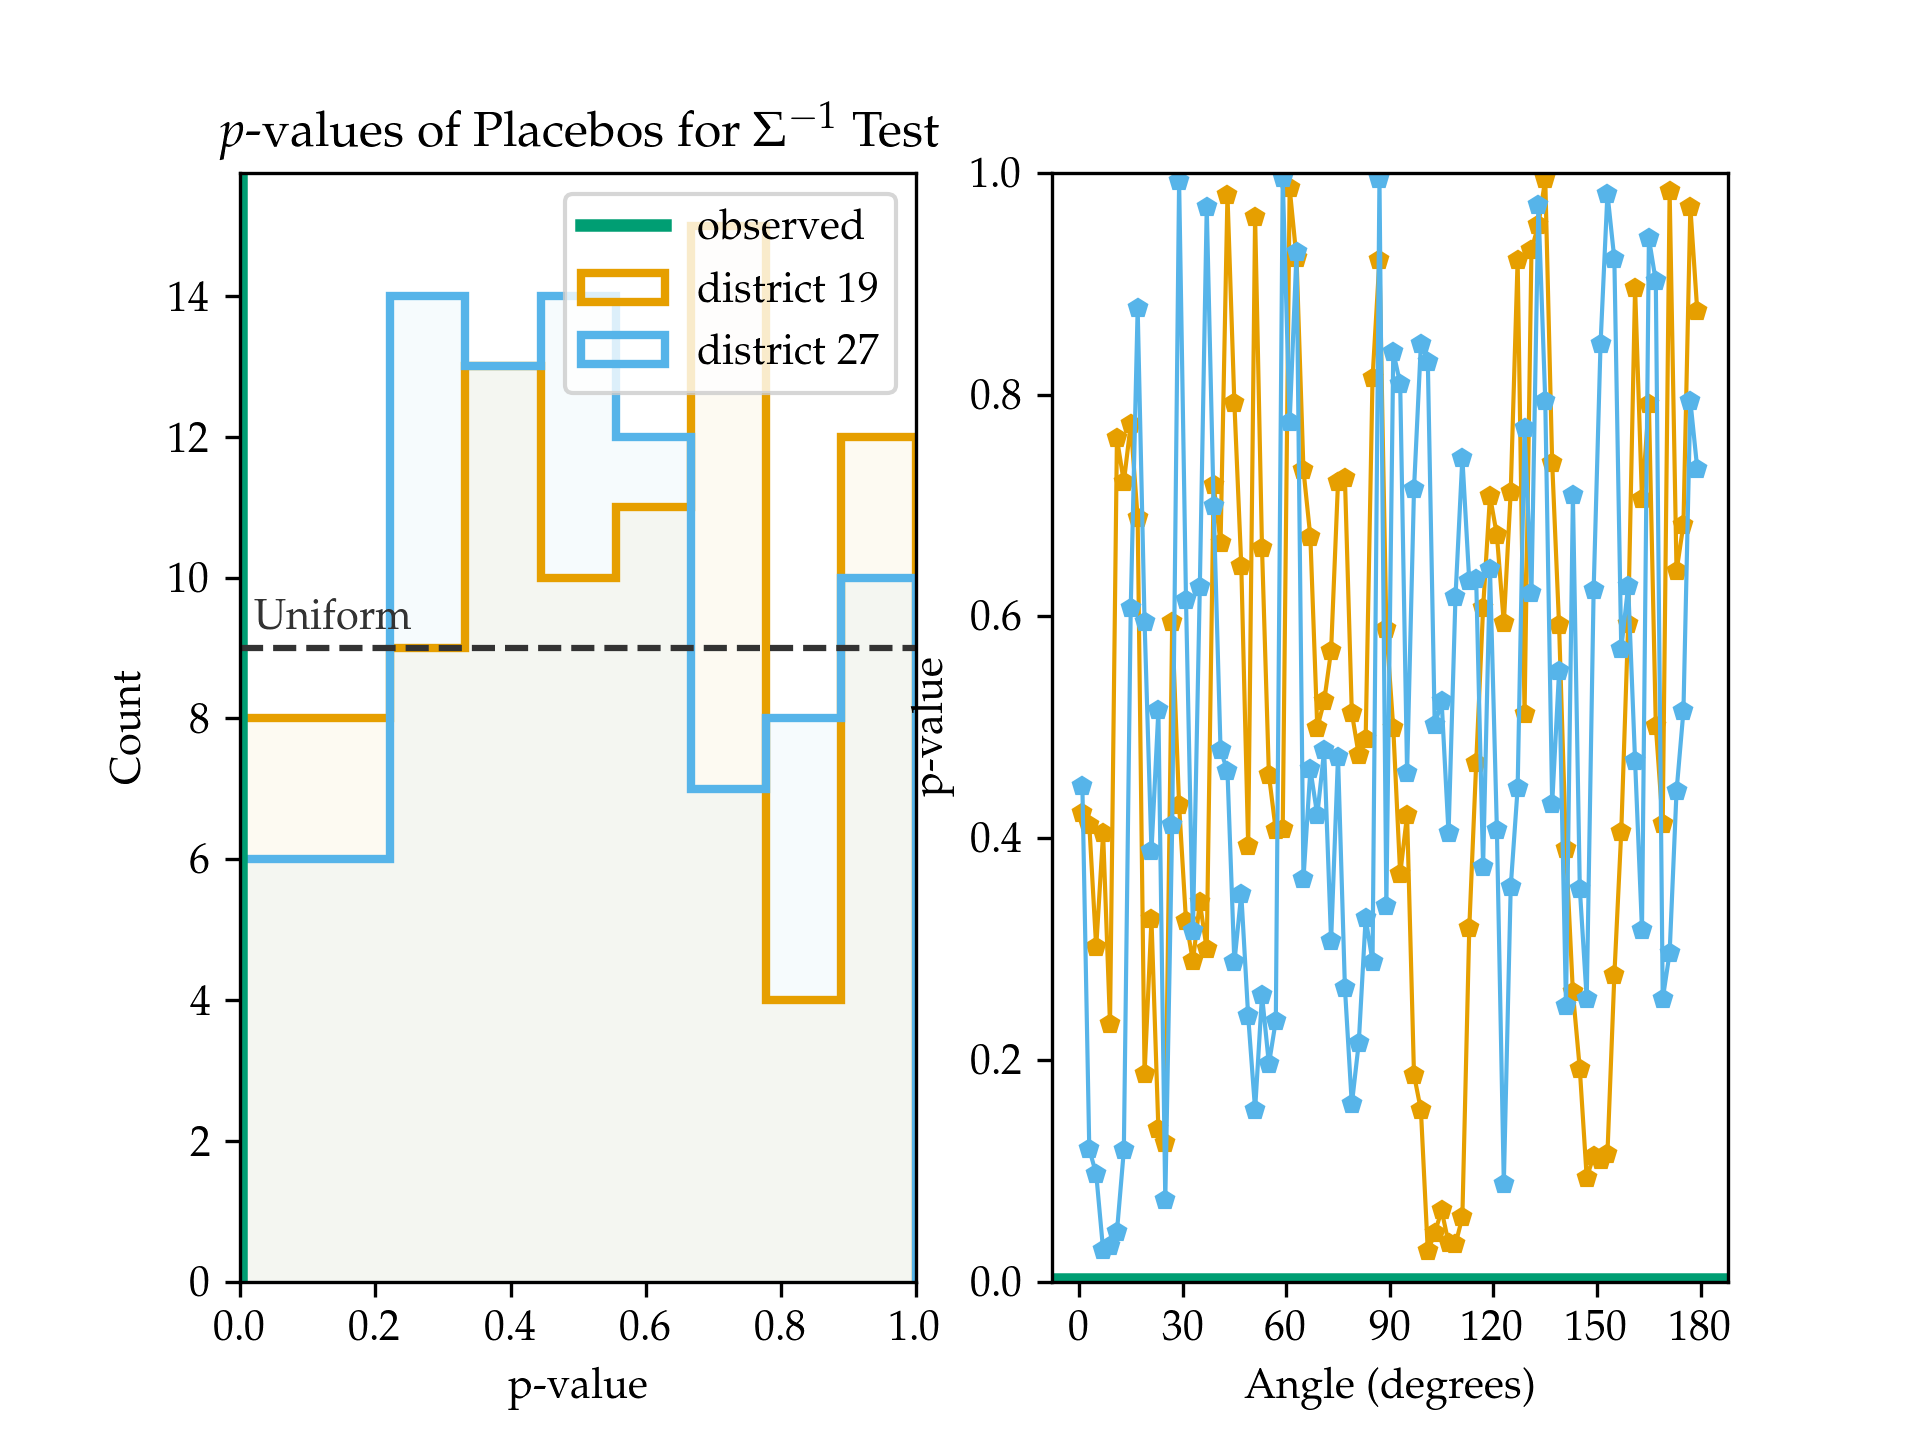
\includegraphics{NYC/NYC_plots/placebo_invvar.png}
\caption{Placebo test for \(\Sigma^{-1}\) test}
\end{figure}

The mLL placebo \(p\)-values show a pronounced bias towards low values.
This confirms our earlier concern that the marginal log-likelihood may be sensitive to features of the data other than the discontinuity at the boundary.
In particular, model misspecification, which is a big concern in spatial models, makes the interpretation of the mLL test unreliable.
Based on this vulnerability, and its manifestation in this example, we do not recommend relying on the likelihood-ratio test.

The \(\chi^2\) test shows more robustness, with some negative bias in district 27, and some positive bias in district 19, which could simply be due to the low effective sample size.
We therefore believe that the \(\chi^2\) test will continue to be reliable under misspecification.
It is only due to its low power that we hesitate to recommend its use in applications where the treatment effect is expected to be fairly homogenous.

Lastly, the inverse-variance placebo \(p\)-values display no obvious bias.
Its high power and robustness to misspecification make a strong argument
for its use in most applications.
    


    	\subsection{pairwise treatment effect (all districts)}\label{pairwise-treatment-effect-all-districts}

\begin{figure}
\centering
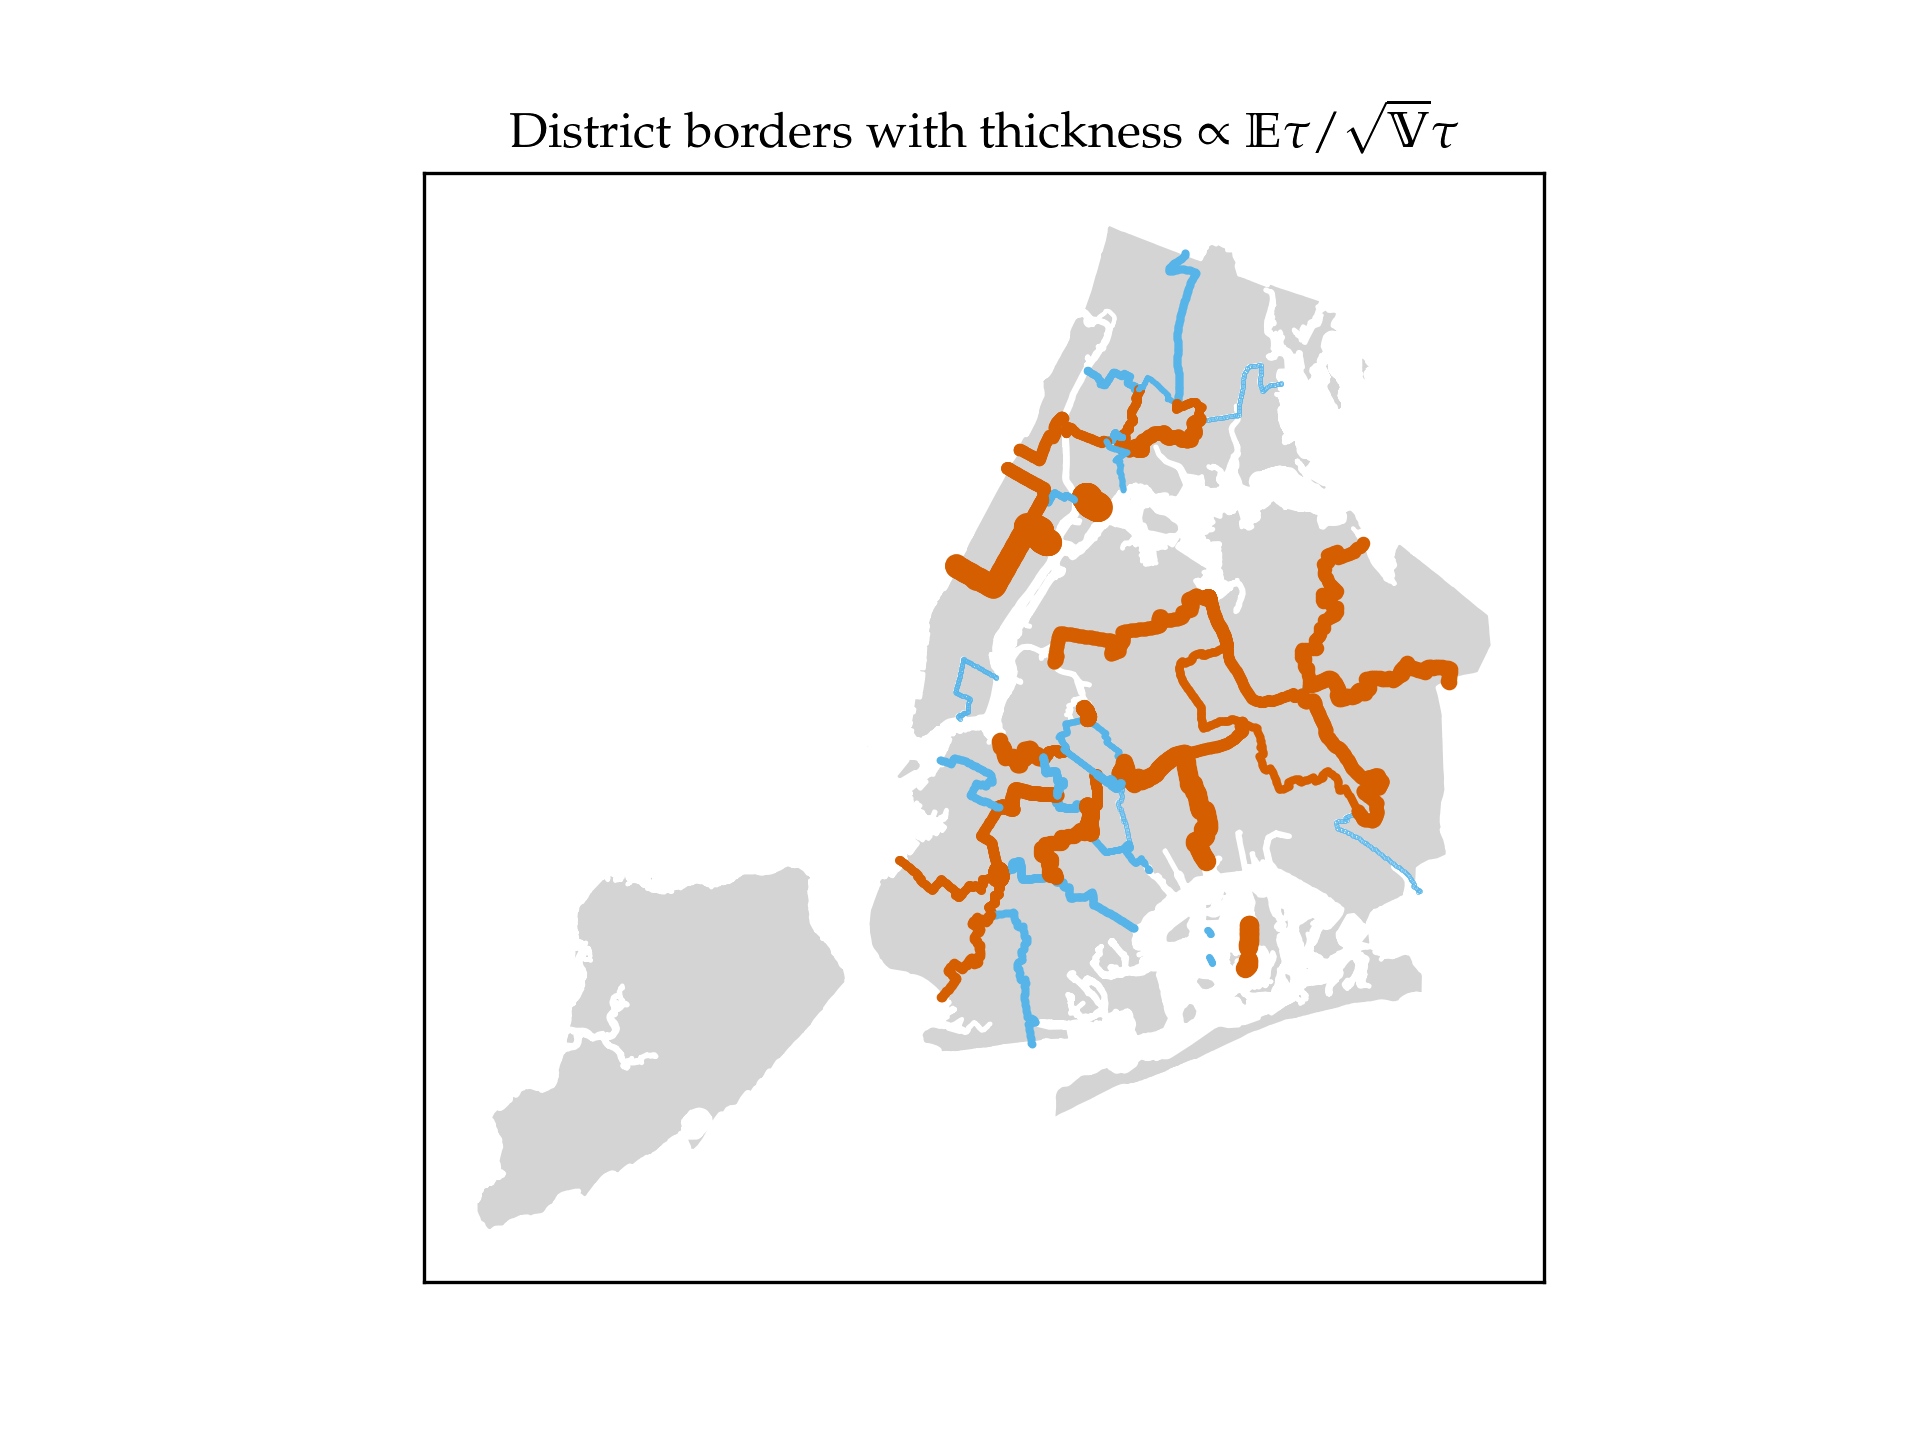
\includegraphics{NYC/NYC_plots/pairwise_multi.png}
\caption{Pairwise effect size between adjacent districts.}
\end{figure}
    


    	\section{Conclusion}\label{conclusion}
    


    	\section{Appendices}\label{appendices}
    


    	\subsection{\texorpdfstring{Posterior mean of \(\hat\beta\)}{Posterior mean of \textbackslash{}hat\textbackslash{}beta}}\label{posterior-mean-of-hatbeta}

\textbf{{[}Derivation of \(\hat{\beta}\) below: should it be in the covariates section? should it be in an appendix? is it too elementary to be in this paper?{]}}

\begin{equation}
\begin{aligned}
    \Sigma_{Y \mid \beta} &\equiv \cov\del{Y \mid \beta } 
        & \text{conditional variance of $Y$} \\
    \cov\del{Y_i , Y_j \mid \beta } &= \sigman^2 \delta_{ij} + k\del{\svec_i,\svec_j} \delta_{\district\sbr{i},\district\sbr{j}} & \text{(block diagonal)}\\
    \Sigma_\beta &\equiv \cov\del{\beta} = \sigma_\beta^2 I_p
        & \text{prior variance of $\beta$} \\
    \Sigma_Y &\equiv \cov\del{Y} = \Sigma_{Y \mid \beta} + D\trans \Sigma_\beta D
        & \text{unconditional variance of $Y$} \\
    T_\beta &= D\trans \Sigma_{Y \mid \beta}^{-1} D + \Sigma^{-1}_\beta 
        & \text{precision matrix of $\beta$} \\
    \hat\beta &= \del{T_\beta^{-1} D} \del{ \Sigma_{Y \mid \beta}^{-1} \del{Y-\mu}}
        & \text{posterior mean of $\beta$}
\end{aligned}
\end{equation}
    


    	\subsection{Calibration of inverse-variance test}\label{calibration-of-inverse-variance-test}

First, let's remind ourselves how the inverse-variance posterior mean estimate was obtained. We will then derive its distribution under the null hypothesis.

\begin{equation}\begin{split}
    \invvar \mid Y_T, Y_C, \sigmaf, \sigman, \ell &\sim \normal\del{\mu_{\invvar \mid Y}, \Sigma_{\invvar \mid Y}} \\
    \mu_{\invvar \mid Y} &\approx \del{\ones\trans \Sigma_{\sentinels \mid Y}^{-1} \mu_{\sentinels \mid Y}} \big/ \del{\ones\trans \Sigma_{\sentinels \mid Y}^{-1} \ones}  \\
    \mu_{\sentinels \mid T} &\equiv \cov\del{g_T(\sentinels), Y_T} \cov\del{Y_T}^{-1}  Y_T \\
    \mu_{\sentinels \mid C} &\equiv \cov\del{g_T(\sentinels), Y_C} \cov\del{Y_C}^{-1}  Y_C \\
    \mu_{\boundary \mid Y} &=  \mu_{\sentinels \mid T} - \mu_{\sentinels \mid C} \\
    \mu_{\invvar \mid Y} &= \del{\ones\trans \Sigma_{\sentinels \mid Y}^{-1} \mu_{\sentinels \mid Y}} \big/ \del{\ones\trans \Sigma_{\sentinels \mid Y}^{-1} \ones}  \\
\end{split}\end{equation}
    


    	Under our parametric null hypothesis \(H_0\), \(Y_T\) and \(Y_C\) are drawn from a single smooth Gaussian process, with no discontinuity at the border.
Their joint covariance is

\begin{equation}
\begin{aligned}
    \cov \del{\begin{pmatrix}Y_T \\ Y_C\end{pmatrix} \mid H_0 } &= \begin{bmatrix}
                        \Sigma_{TT} & \Sigma_{TC} \\
                        \Sigma\trans_{TC} & \Sigma_{CC}
                    \end{bmatrix}\,\text{where} \\
    \Sigma_{TT} &\equiv K_{TT} + \sigman^2 I_{n_T} \\
    \Sigma_{CC} &\equiv K_{CC} + \sigman^2 I_{n_C} \\
    \Sigma_{TC} &\equiv K_{TC}
\end{aligned}
\end{equation}

where the entries of \(K_{TT}\), \(K_{CC}\) and \(K_{TC}\) are obtained simply be evaluating the Gaussian process kernel for each pair of points within and between the treatment and control regions.
The predicted mean outcomes at the sentinels \(\mu_{\sentinels \mid T}\) and \(\mu_{\sentinels \mid T}\) are obtained by left-multiplying \(Y_T\) and \(Y_C\) by matrices that are deterministic functions of the unit locations and the hyperparameters

\begin{equation}
\begin{split}
    A_T &\equiv \cov\del{g_T(\sentinels), Y_T} \cov\del{Y_T}^{-1} = K_{\sentinels T} \Sigma_{TT}^{-1} \,\text{, and} \\
    A_C &\equiv \cov\del{g_C(\sentinels), Y_C} \cov\del{Y_C}^{-1} = K_{\sentinels C} \Sigma_{CC}^{-1}\,.
\end{split}
\end{equation}

where we dropped the explicit conditioning on the null hypothesis for readability.
    


    	The joint distribution of \(\mu_{\sentinels \mid T}\) and \(\mu_{\sentinels \mid T}\) is consequently also multivariate normal with mean zero and covariance

\begin{equation}
    \cov \del{\begin{pmatrix}A_T Y_T \\ A_C Y_C \end{pmatrix} \mid H_0 } = \begin{bmatrix}
                        A_T \Sigma_{TT} A_T\trans & A_T \Sigma_{TC} A_C\trans \\
                        \del{A_T \Sigma_{TC} A_C \trans}\trans & A_C \Sigma_{CC} A_C\trans
                    \end{bmatrix}
\end{equation}

Continuing in this fashion, \(\mu_{\boundary \mid Y}\) is yet another zero-mean multivariate normal with covariance
    


    	\begin{equation}
\begin{split}
    \cov \del{\mu_{\boundary \mid Y} \mid H_0} &= \cov{ A_T Y_T - A_C Y_C } \\
        &= A_T \Sigma_{TT} A_T\trans + A_C \Sigma_{CC} A_C\trans - A_T \Sigma_{TC} A_C\trans -  \del{A_T\Sigma_{TC} A_C\trans}\trans
\end{split}
\end{equation}
    


    	Weighted mean estimators are linear transformation of \(\mu_{\boundary \mid Y}\), and so under \(H_0\), they are normally distributed with mean zero.
For a weight vector \(\vvec\), its variance is given by

\begin{equation}
\begin{aligned}
    \var\del{\bar{\tau}^\vvec \mid H_0} &= \cov\del{ \frac{\vvec \trans \mu_{\boundary \mid Y}}{\ones_{n_{\sentinels}}\trans \vvec}} \\
    &= \frac{\vvec \trans \cov \del{\mu_{\boundary \mid Y}} \vvec}{\del{\ones_{n_{\sentinels}}\trans \vvec}^2}
    \,.
\end{aligned}
\end{equation}
    


    	From this null distribution the \(p\)-value follows:

\begin{equation}
    \Pr\del{ \abs{\bar{\tau}^\vvec} > \abs{\bar{\tau}_{obs}^\vvec} \mid H_0} = 2 \Phi\del{ -\frac{\abs{\bar{\tau}_{obs}^\vvec}}{\sqrt{\var\del{\bar{\tau}^\vvec \mid H_0}}} }\,.
\end{equation}

Our calibrated inverse-variance test is the special case of this final step where the weights are chosen to be \(\vvec = \Sigma^{-1}_{\boundary \mid Y} \ones_{n_{\sentinels}}\).
    



    % Add a bibliography block to the postdoc
    
    
	\bibliographystyle{ametsoc2014}
	\bibliography{GeoRDD}

    
    \end{document}
